\documentclass[11pt,twoside,a4paper]{article}
\usepackage{a4wide,xspace,subfigure,amsmath,amssymb,multicol,graphicx,lscape,color}
\usepackage{epic,eepic,sidecap,paralist,verbatim,upquote}
\usepackage[margin=2.5cm]{geometry}
\usepackage[small]{caption}
\usepackage[colorlinks=true,citecolor=darkblue,linkcolor=darkblue,
            urlcolor=darkblue]{hyperref}
\usepackage{bookmark}
\protect{\renewcommand{\arraystretch}{1.2}}
\pagestyle{myheadings}
\pagenumbering{arabic}
\protect{\setcounter{page}{1}}
\raggedbottom
\tolerance=10000
\setlength{\parskip}{0.5em}

\definecolor{Mygrey}{gray}{0.975}
\definecolor{darkblue}{rgb}{0.0,0.0,0.55}

%% Margin references to books
\newcommand{\MD}[1]{\marginpar{\raggedright\bf MD\ #1}}
\newcommand{\DA}[1]{\marginpar{\raggedright\bf DA\ #1}}
\newcommand{\PP}[1]{\marginpar{\raggedright\bf P\ #1}}
\newcommand{\TS}[1]{\marginpar{\raggedright\bf TS\ #1}}
\newcommand{\EH}[1]{\marginpar{\raggedright\bf EH\ #1}}

%% Grey boxes and other shortcuts.
\newcommand{\bx}[1]{\noindent\fcolorbox{black}{Mygrey}{\parbox{\textwidth}{#1}}\\[-1mm]}
\newcommand{\bxc}[1]{\noindent\fcolorbox{black}{Mygrey}{\parbox{\textwidth}{\centering{}#1}}\\[-1mm]}
\newcommand{\bqx}[1]{\noindent\fcolorbox{black}{Mygrey}{\parbox[t]{15cm}{#1}}\\[-2mm]}
\newcommand{\Eref}[1]{Equation~(\ref{eq:#1})}
\newcommand{\eref}[1]{equation~(\ref{eq:#1})}
\newcommand{\Sec}[1]{Section~\ref{sec:#1}}
\newcommand{\question}{\noindent\textbf{Question:}\xspace}
\newcommand{\labtitle}[2]{\begin{center}\Huge{Laboratory #1}\\\Large{#2}\end{center}}

%% Matlab
\newcommand{\Mlab}{\textsc{Matlab}\xspace}
\newcommand{\Minput}[1]{\newline\indent\indent\texttt{>> #1}}
\newcommand{\Matlab}[3]{\\[2mm]\indent\indent\begin{minipage}{12cm}{
        \setlength{\parindent}{5mm}
        \noindent\texttt{>> #1}\nopagebreak[4]\\
        \noindent\texttt{#2 = }\nopagebreak[4]\\[2mm]
        \indent\indent\parbox{5cm}{\texttt{#3}}}\end{minipage}\\[2mm]}
\newcommand{\Moutput}[2]{\newline\indent\indent\texttt{#1 = }\newline
        \indent\indent\indent\indent\texttt{#2}\newline}
\newcommand{\qu}{\textquotesingle}

%% Math
\newcommand{\bv}[1]{\mbox{{\bf #1}}}
\newcommand{\Grad}{\mbox{\boldmath $\nabla$}}
\newcommand{\Div}{\Grad\!\cdot}
\newcommand{\Curl}{\Grad\!\times}
\newcommand{\delsq}{\nabla^2}
\newcommand{\mean}[1]{\left\langle{#1}\right\rangle}
\newcommand{\infd}{\textrm{d}}
\newcommand{\diff}[2]{\frac{\infd #1}{\infd #2}}
\newcommand{\difftwo}[2]{\frac{\infd^2 {#1}}{\infd {#2}^2}}
\newcommand{\pdiff}[2]{\frac{\partial #1}{\partial #2}}
\newcommand{\pdiffcon}[3]{\left(\frac{\partial #1}{\partial #2}\right)_{#3}}
\newcommand{\pdifftwo}[2]{\frac{\partial^2 {#1}}{\partial {#2}^2}}
\newcommand{\pdifftwomix}[3]{\frac{\partial^2 {#1}}{\partial {#2}\,\partial {#3}}}
\newcommand{\vel}{\bv{v}}
\newcommand{\expu}[1]{\textrm{e}^{#1}}
\newcommand{\ehat}{\bv{e}}

\renewcommand{\thefootnote}{\fnsymbol{footnote}}

% make autoref references nicer
\makeatletter
\def\tagform@#1{\maketag@@@{\ignorespaces#1\unskip\@@italiccorr}}
\let\orgtheequation\theequation
\def\theequation{(\orgtheequation)}
\makeatother

\newcommand{\runtitle}{Fourier analysis}
\markboth{\runtitle}{\runtitle}
\title{DTP lecture notes: \\
  Fourier analysis of time-series and functions}
\author{Prof.~Richard Katz}

\begin{document}

\maketitle{}

\section{Fourier Series}
\label{sec:fourierseries}

\paragraph{In this section} we'll learn about how a finite, periodic
function can be expressed as a sum of sine and cosine functions of
different amplitudes and frequencies. We'll learn how to calculate all
of the terms of that sum.  We'll be doing only analytical maths in
this lecture; no \Mlab stuff.  Two books that should be helpful for
alternative explanations and going beyond the lectures are
\begin{itemize}
\item Seeley, RT; \underline{An introduction to Fourier series and
    integrals}, W.A. Benjamin (New York), 1996.
\item Riley, Hobson, and Bence; \underline{Mathematical methods for
    physics and engineering}, Cambridge University Press (Cambridge),
  2006.
\end{itemize}
Both of these are available through the Oxford library system.

\subsection{Aside: coordinate systems and orthogonality}

We're familiar with the concept of Cartesian, three dimensional space:
any point can be described as the sum of three independent basis
vectors, pointing in each of the three independent directions,
\begin{equation}
  \label{eq:vec}
  \bv{V} = c_1\ehat_1 + c_2\ehat_2 + c_3\ehat_3 = \sum_{j=1}^3 c_j\ehat_j, 
\end{equation}
where
\begin{align}
  \ehat_1 &=
  \left[\begin{array}{c}
    1 \\ 0 \\ 0
  \end{array}\right],&
  \ehat_2 &=
  \left[\begin{array}{c}
    0 \\ 1 \\ 0
  \end{array}\right],&
  \ehat_3 &=
  \left[\begin{array}{c}
    0 \\ 0 \\ 1
  \end{array}\right]. \nonumber
\end{align}
The essential property of these basis vectors is that they are
\textit{mutually orthogonal}:
\begin{equation}
  \label{eq:orthog}
  \ehat_i\cdot\ehat_j=
  \begin{cases}
    1 & \text{if }i=j,\\
    0 & \text{if }i\ne j.
  \end{cases}
\end{equation}
For example, basis vector 1 contains no amount of basis vector 2; each
basis vector is entirely independent of the others.  This means that
we can determine the $y$-value of a vector independently of the $x$
and $z$-values.  Furthermore, any point in Cartesian space has a
\textit{unique} set of coordinates.  It is therefore true that any
vector in Cartesian space can be \textit{decomposed} into a sum of
basis vectors, as we did above.  To find the, say, $x$-component of a
vector, one need only take the dot-product of the vector with the
basis vector in the $x$-direction:
\begin{displaymath}
  \bv{V}\cdot\ehat_1 = c_1.
\end{displaymath}
This is a trivial example, but it demonstrates a concept that is
important in understanding Fourier series.

\textit{It turns out that we can decompose functions in a manner
  similar to vectors}.  Just as a general vector was decomposed into a
set of simpler basis vectors, a function can be decomposed into a set
of basis functions.  We'll see how below.

\subsection{Periodic functions: a general definition}

A periodic function is one that repeats, identically, once each
period, from $-\infty$ to $+\infty$.  If the function is denoted by
$f(t)$ and the period is $T$, then the following equation defines
a periodic function
\begin{equation}
  \label{eq:defperiodic}
  f(t+T) = f(t).
\end{equation}

\begin{SCfigure}[0.5][tb]
  \centering
  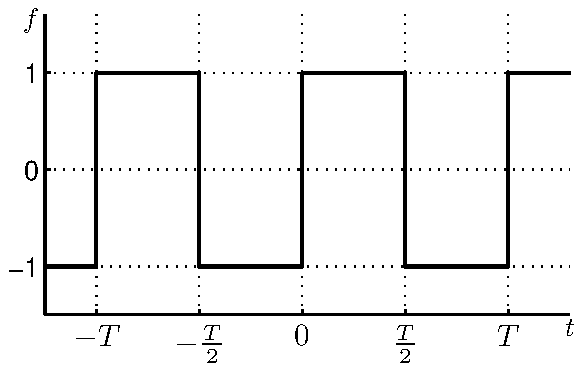
\includegraphics[height=2in]{../figs/L14/SquareWave}
  \caption{A square wave with period $T$ and unit amplitude, as
    described by \autoref{eq:squarewave}.  \vspace{1cm}}
  \label{fig:sqwave}
\end{SCfigure}

One obvious example of a periodic function is $\cos t$; it has a
period of $T=2\pi$, and of course $\cos(t)=\cos(t+2\pi)$, which
satisfies \autoref{eq:defperiodic}. Here's another example of a
periodic function:
\begin{equation}
  \label{eq:squarewave}
  f(t) =
  \begin{cases}
    -1 & \text{for }-T/2\le t<0,\\
    +1 & \text{for }0\le t<T/2.
  \end{cases}
\end{equation}
This is called a square wave, and is represented in
\autoref{fig:sqwave}.

\subsection{The Fourier series}

Amazing but true: any periodic function\footnote{\raggedright Terms
  and conditions apply, see Riley, Hobson, \& Bence,
  \underline{Mathematical Methods for Physics and Engineering},
  Cambridge University Press.}, including the one in
\autoref{fig:sqwave}, can be represented by the sum of a series of
sines and cosines.  For a periodic function $g(t)$ with period $T$,
this series is
\begin{equation}
  \label{eq:fourierseries}
  g(t) = a_0 + \sum_{r=1}^\infty
  \left[a_r\cos\left(\frac{2\pi r}{T}t\right) +
    b_r\sin\left(\frac{2\pi r}{T}t\right)\right].
\end{equation}
Some remarks about this important equation:
\begin{itemize}
\item Compare \autoref{eq:fourierseries} to \autoref{eq:vec}: whereas
  a vector is composed of different quantities of each basis vector, a
  periodic function is composed of different quantities of each sine
  and cosine in the series.  The quantities $c_1,c_2,c_3$ are the
  \textit{coordinates} of a point in \textit{physical space}. The
  quantities $a_0,a_1,...$ and $b_1,b_2,...$ are the coordinates of a
  function in \textit{frequency space}.
\item The series contains an infinite number of terms; calculating all
  of them is impractical.  Often, we will sum up a large number, but
  not all the terms.  Doing this changes \autoref{eq:fourierseries}
  into an approximation, rather than an equality.
\item The $a_0$ term in the equation is a constant and represents the
  mean of the function $g(t)$.  Since $g$ is periodic, we can
  calculate the mean by averaging over one period
  \begin{equation}
    \label{eq:a0term}
    a_0 = \frac{1}{T}\int_{t_0}^{t_0+T}g(t)\,\infd t.
  \end{equation}
  There is no $b_0$ term in the series because $\sin(0)=0$.
\item The coefficients $a_1,a_2,...$ and $b_1,b_2,...$ are constants
  to be determined.  Fortunately, it is possible to calculate them,
  because each term in the series is \textit{mutually orthogonal},
  just as were the basis vectors in \autoref{eq:orthog}:
  \begin{subequations}
    \label{eq:orthogcond}
    \begin{align}
      \int_{t_0}^{t_0+T}\cos\left(\frac{2\pi r}{T}t\right)
      \sin\left(\frac{2\pi s}{T}t\right)\,\infd t&=0 \;\;\;\;\;
      \text{for all
        integers $r$ and $s$},\\
      \int_{t_0}^{t_0+T}\cos\left(\frac{2\pi r}{T}t\right)
      \cos\left(\frac{2\pi s}{T}t\right)\,\infd t&=
      \begin{cases}
        T/2 & \text{for $r=s$} \\
        0 & \text{for $r\ne s$}
      \end{cases},\\
      \int_{t_0}^{t_0+T}\sin\left(\frac{2\pi r}{T}t\right)
      \sin\left(\frac{2\pi s}{T}t\right)\,\infd t&=
      \begin{cases}
        T/2 & \text{for $r=s$} \\
        0 & \text{for $r\ne s$}
      \end{cases}.
    \end{align}
  \end{subequations}
  These relations indicate that each entry in the series adds a unique
  contribution that cannot be obtained by any other entry.
\end{itemize}

\subsection{Applying the orthogonality conditions}
To obtain values for the Fourier coefficients, we need a means to
isolate and solve for them.  The orthogonality conditions
\eqref{eq:orthogcond} provide a means.  To see this, take
\autoref{eq:fourierseries}, multiply both sides of the equation by,
say, $\cos(2\pi s t/T)$, and integrate over one period.  This gives
\begin{multline}
  \label{eq:applyorthog}
  \int_{t_0}^{t_0+T}\cos\left(\frac{2\pi s}{T}t\right)g(t)\,\infd t = \\ 
  \int_{t_0}^{t_0+T}\cos\left(\frac{2\pi s}{T}t\right)\left\{
    a_0 + \sum_{r=1}^\infty
    \left[a_r\cos\left(\frac{2\pi r}{T}t\right) +
      b_r\sin\left(\frac{2\pi r}{T}t\right)\right] \right\}\,\infd t
\end{multline}
Now focus on the right-hand side of \autoref{eq:applyorthog}. We can
bring the integral into the summation and write the RHS as
\begin{align}
  &a_0\int_{t_0}^{t_0+T}\cos\left(\frac{2\pi s}{T}t\right)\,\infd t\,+ &
  &\text{[term 1]} \nonumber\\
   &\sum_{r=1}^\infty\left[a_r\int_{t_0}^{t_0+T}\cos\left(\frac{2\pi
        s}{T}t\right)\cos\left(\frac{2\pi r}{T}t\right)\,\infd
    t\right] + & &\text{[term 2]}\nonumber\\
    &\sum_{r=1}^\infty\left[b_r\int_{t_0}^{t_0+T}\cos\left(\frac{2\pi s}{T}t\right)
    \sin\left(\frac{2\pi r}{T}t\right)\,\infd t \right]. & &\text{[term
    3]} \nonumber
\end{align}
First consider [term 1]: integrating cosine over a full period (or $s$
full periods) gives zero by inspection.  Now [term 3]: orthogonality
condition \autoref{eq:orthogcond}a clearly applies, so this term is
also zero.  Finally, consider [term 2]: this matches with
orthogonality condition \autoref{eq:orthogcond}b; this term is only
non-zero if $r=s$.  This means that all terms with $r\ne s$ in the
summation are zero!  We can therefore discard the summation!

Using these three simplifications, we can rewrite
\autoref{eq:applyorthog} as
\begin{equation}
  \label{eq:cosinecoef}
  a_s\frac{T}{2} = \int_{t_0}^{t_0+T}\cos\left(\frac{2\pi s}{T}t 
  \right)g(t)\,\infd t,
\end{equation}
which is a formula for calculating cosine coefficient, $a_s$.  We can
apply a similar method (multiply eqn.~\eqref{eq:fourierseries} by
$\sin(2\pi s t/T)$ and integrate over one period) to obtain the sine
coefficients $b_s$.

\subsection{Calculating the Fourier coefficients} 
In the previous section, we used the orthogonality conditions to
derive the following formulae for the coefficients
\begin{subequations}
  \label{eq:coefrecipe}
  \begin{align}
    a_r &= \frac{2}{T}\int_{t_0}^{t_0+T}g(t)
      \cos\left(\frac{2\pi r}{T}t\right)\,\infd t, \\
    b_r &= \frac{2}{T}\int_{t_0}^{t_0+T}g(t)
      \sin\left(\frac{2\pi r}{T}t\right)\,\infd t.
  \end{align}
\end{subequations}
(These formulae are examinable).

\autoref{eq:coefrecipe} can be used blindly to compute the
coefficients of a Fourier series, but as usual, a bit of care will
save us work.  This comes from noting that $\sin$ is an \textit{odd
  function} while $\cos$ is an \textit{even function}:
\begin{align}
  \sin(-x) &= -\sin(x), & &\text{therefore odd},\nonumber\\
  \cos(-x) &= \cos(x),  & &\text{therefore even}.\nonumber
\end{align}

If the function $g(t)$ is odd, then we can infer that all $a_r$ must
equal zero, since these are the coefficients of $\cos$ terms, which
are even (and therefore couldn't contribute to an odd function).  If
$g(t)$ is even, then all $b_r$ must equal zero.

\paragraph{A recipe for calculating the Fourier series of a periodic
  function}
\begin{enumerate}
\item Determine the period $T$ of the function. Choose a starting
  point $t_0$, usually the beginning of a period of oscillation.
\item Calculate the mean of the function over one period, and assign
  this value to $a_0$.
\item Ascertain whether the function is even, odd, or neither.
\item Use \autoref{eq:coefrecipe} to calculate the required
  coefficients depending on your result from the previous step.
\item Assemble the coefficients with their respective sine and cosine
  functions and frequencies, and write down the resulting Fourier
  series. 
\item Check your result!
\end{enumerate}

\subsection{A worked example}

Let's calculate a Fourier series of the square wave from
\autoref{fig:sqwave} and \autoref{eq:squarewave}.
\begin{enumerate}
\item By construction, the period of the function is $T$.  Let's
  choose $t_0=-T/2$ because it is the beginning of a cycle.
\item By inspection of \autoref{fig:sqwave}, we can see that the mean
  of this function is zero, and hence $a_0=0$.
\item By inspection of \autoref{fig:sqwave}, we can see that the
  function is odd.  We can therefore take $a_r=0$ for all $r>0$.
\item We now use \autoref{eq:coefrecipe} to determine $b_r$:
  \begin{align}
    b_r &= \frac{2}{T}\int_{-T/2}^{T/2}g(t)\sin\left(\frac{2\pi
        r}{T}t\right)\,\infd t && \text{by using \autoref{eq:coefrecipe}b}\nonumber\\
    &= \frac{2}{T}\left[\int_{-T/2}^{0}(-1)\sin\left(\frac{2\pi
        r}{T}t\right)\,\infd t + \int_{0}^{T/2}(1)\sin\left(\frac{2\pi
        r}{T}t\right)\,\infd t\right] && \text{split the integral into
                                         two parts}\nonumber\\
    &= \frac{4}{T}\int_{0}^{T/2}g(t)\sin\left(\frac{2\pi
        r}{T}t\right)\,\infd t&& \text{by exploiting symmetry about $t=0$}\nonumber\\
    &= \frac{4}{T}\int_{0}^{T/2}\sin\left(\frac{2\pi
        r}{T}t\right)\,\infd t&& \text{by substituting for $g(t)$}\nonumber\\
    &= -\frac{4}{T}\left(\frac{T}{2\pi r}\right)\left[\cos\left(\frac{2\pi
          r}{T}t\right)\right]_{0}^{T/2}&& \text{by integration}\nonumber\\
    &= -\frac{2}{\pi r}[\cos(\pi r) - \cos(0)] = \frac{2}{\pi r}[1 -
    (-1)^r] && \text{by algebra}\nonumber\\
    &=
    \begin{cases}
      \frac{4}{\pi r} & \text{ for $r$ odd},\\
      0 & \text{for $r$ even}.
    \end{cases}&& \text{by splitting into cases}\nonumber
  \end{align}
\item Hence we can assemble the Fourier series as 
  \begin{displaymath}
    g(t) = \frac{4}{\pi}\left[\sin(\omega t) + \frac{\sin(3\omega
        t)}{3} + \frac{\sin(5\omega t)}{5} + ...\right],
  \end{displaymath}
  where $\omega = 2\pi/T$ is the angular frequency.
\item To check our work we plot the solution in 
  \autoref{fig:sqwaveFS}.
\end{enumerate}

\begin{figure}[tb]
  \centering
  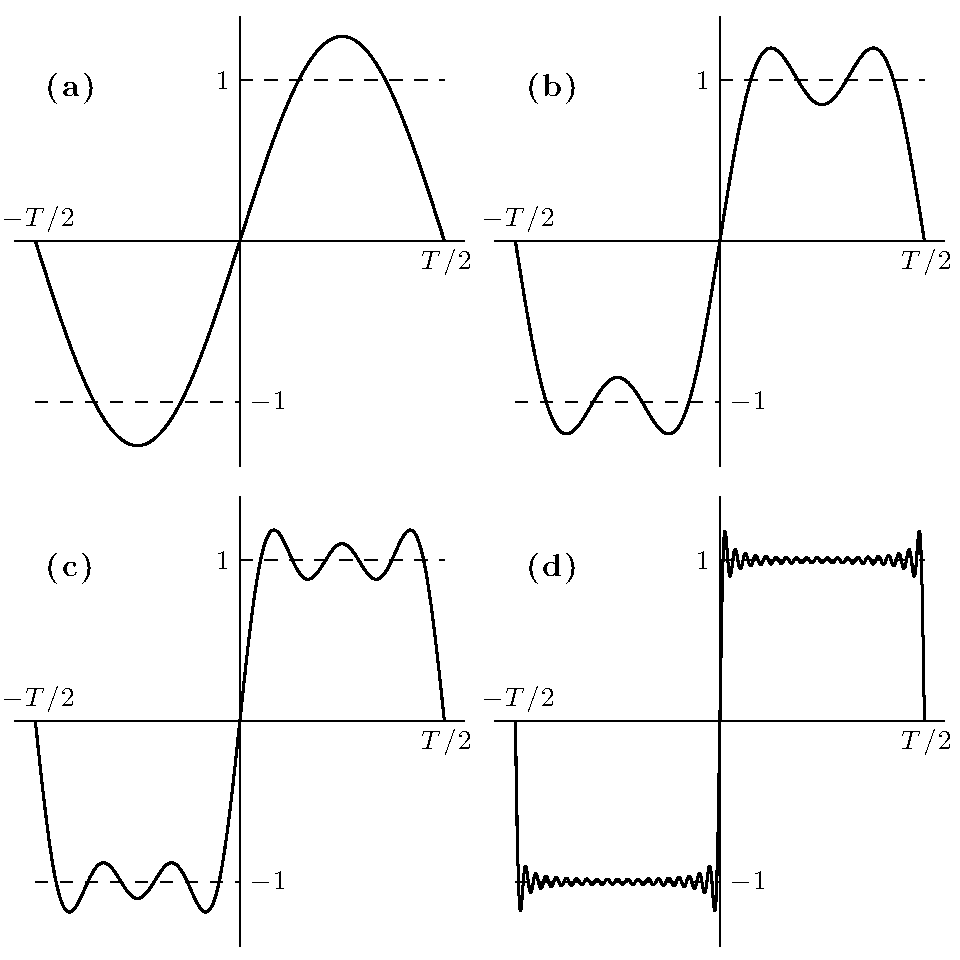
\includegraphics[width=4.5in]{../figs/L14/FourierSeriesConvergence}
  \caption{The convergence of a Fourier series expansion of a
    square-wave function, including \textbf{(a)} one term ($r=1)$,
    \textbf{(b)} two terms ($r=1,3$), \textbf{(c)} three terms
    ($r=1,3,5$), \textbf{(d)} twenty terms ($r=1,3,5,7,...,39$).}
  \label{fig:sqwaveFS}
\end{figure}

\subsection{Fourier series of discontinuous functions}

While it is possible to find the Fourier series of discontinuous
functions (we did so in the example above), the series will always
``overshoot'' the function at the discontinuities.  Such overshoot is
evident in \autoref{fig:sqwaveFS}.  It is called the \textit{Gibb's
  phenomenon}, and it does not disappear no matter how many terms we
of the series that we sum. For functions without discontinuities the
Fourier series generally does not have any problems.

%%%%%%%%%%%%%%%%%%%%%%%%%%%%%%%%%%%%%%%%%%%%%%%%%

\section{Discrete Fourier Series and Power Spectra}
\label{sec:dft1}

\paragraph{In this section} We learn about how the same concepts that
were used to develop the Fourier series can be applied to the analysis
of time-series data.  We'll also learn how the resulting series can be
converted into a \textit{spectrum}, a useful plot that can give
fundamental information about the processes that are reflected in the
time-series.

\subsection{From time-series to radian-series}

\DA{pp. 268--272} Let's consider a time-series $\bv{y}$ consisting of
$N$ observations, with an equal spacing in time $\Delta t$, starting
from time zero (if our time-series were not equally spaced, we could
use interpolation to obtain an equally spaced series that represents
the data). Our goal is to somehow apply to this time-series a
\textit{Fourier analysis} like what we saw in the last lecture.

We can represent the time-series as
\begin{align}
  \bv{y} &= y_0,\,y_1,\,y_2,\,y_3,\,...\,y_{N-1},\nonumber\\
  \bv{t} &= t_0,\,t_1,\,t_2,\,t_3,\,...\,t_{N-1}.\nonumber
\end{align}
Furthermore, since we wish to apply Fourier analysis, we must make a
\textit{periodic extension} of the series, to turn it into a periodic
function of time that extends from $-\infty$ to $+\infty$ (analogous
to our periodic functions from the last lecture).  This means that
stepping past the end of our time-series should take us back to the
beginning; we have wrapped the time-series around a circle, as shown
in \autoref{fig:circleseries}.

\begin{SCfigure}[1][bh]
  \centering
  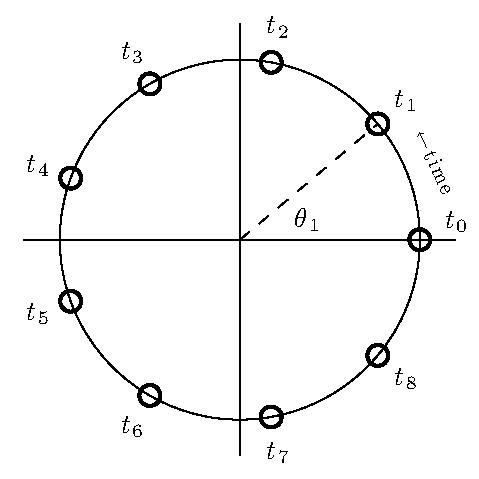
\includegraphics[height=2.5in]{../figs/L15/CircularTimeseries}
  \caption{A time-series with $N=9$ entries wrapped around a circle,
    making it periodic. Each time $t_j$ corresponds to a angle
    $\theta_j$. \vspace{1cm}}
  \label{fig:circleseries}
\end{SCfigure}

The time-series shown in \autoref{fig:circleseries} has $N=9$
entries. The total time to complete the trip around the circle and
arrive back at the initial point is period $T=N\Delta t$. This
motivates us to convert the time-series into \textit{radians} as
follows
\begin{displaymath}
  \theta_j = \frac{2\pi t_j}{T}.
\end{displaymath}
Since our entries are regularly spaced in time, we can substitute $t_j
= j\Delta t$, as well as our definition for the period $T$ to obtain
\begin{equation}
  \label{eq:radvar}
  \theta_j = \frac{2\pi j}{N}
\end{equation}
and we can rewrite our time-series as 
\begin{align}
  \bv{y} &= y_0,\,y_1,\,y_2,\,y_3,\,...\,y_{N-1},\nonumber\\
  \boldsymbol{\theta} &= \theta_0,\,\theta_1,\,\theta_2,\,
  \theta_3,\,...\,\theta_{N-1}.\nonumber
\end{align}
Here we have replaced the time-coordinate of our series with a
corresponding angle in radians, such that the series becomes periodic.
By construction $\theta_0=0$ and $\theta_N=2\pi$.  This makes it
amenable to Fourier analysis.

\subsection{Discrete Fourier series}

We now posit a new type of Fourier series that decomposes a
\textit{discrete} rather than continuous signal.  Instead of a
periodic function, we're going to analyse a series of discrete
points in a time-series.  Similar to \autoref{eq:fourierseries}, we
use the equation
\begin{equation}
  \label{eq:discretefourier_1}
  \bv{y} = \sum_k[\alpha_k\cos(k\boldsymbol{\theta}) + 
  \beta_k\sin(k\boldsymbol{\theta})]
\end{equation}
to represent the discrete Fourier series. As before, $\alpha_k$ and
$\beta_k$ are unknown coefficients, and $k$ is an integer, called the
\textit{harmonic number}. For $k=0$, the sine term drops out and the
cosine term becomes a constant $\alpha_0$; this is the mean of the
time-series.  We can substitute our discrete values of $\theta$ from
\autoref{eq:radvar} to obtain
\begin{equation}
  \label{eq:discretefourier_2}
  y_j = \sum_k\left[\alpha_k\cos\left(\frac{2\pi k}{N}j\right) + 
    \beta_k\sin\left(\frac{2\pi k}{N}j\right)\right].
\end{equation}
Here the integer index $j$ has replaced time $t$ as the independent
variable. The angular frequency $2\pi k/N$ has replaced $\omega$.

For the series represented by \autoref{eq:discretefourier_2}, there
are always an odd number of unknown coefficients.  This can be seen by
considering that the unknown coefficients of the series come in pairs
$(\alpha_k,\beta_k)$ except for at $k=0$, where there is only one
coefficient, $\alpha_0$.  To solve for the unknown coefficients, we
must have an equal number of data points in our time-series;
\textit{hence $N$ must be odd}\footnote{A modified version of
  \autoref{eq:discretefourier_2} can be used to compute the discrete
  Fourier series of a time-series with $N$ even.  We will not consider
  that modification here.}.  We can accommodate this by interpolation,
or by simply dropping the last entry before analysing the series.

The sine and cosine oscillations with $k=1$ represent the longest
period that we can resolve in our analysis of the time-series.  In
fact, they represent the oscillations with discrete period $N$, which
correspond to period $T$.

At larger harmonic number $k$, the frequency of the corresponding
oscillation grows (in other words, the period shrinks).  What is the
largest frequency (smallest period) that can be resolved?
Equivalently, what is the maximum harmonic number $k$ in the summation
in \autoref{eq:discretefourier_2}? Think back to what you learned
about \textit{aliasing} in problem 4 of Laboratory 5 from this term:
to represent an oscillation, you need to \textit{sample it at least
  twice per period}.  This means that for a given sampling rate
$\Delta t$, the smallest period that you can hope to capture is the
one with a $T_\text{min}=2\Delta t$, corresponding to a harmonic
number $k_\text{max}=N/2$.  This value of $k$ is known as the
\textit{Nyquist frequency}; it is the largest frequency that we can
resolve in a time-series. In practise, for $N$ odd, the best we can do
is $T_\text{min}=2\Delta t N/(N-1)$ or
\begin{displaymath}
  k_\text{max} = \frac{N-1}{2}.
\end{displaymath} 
Using these limits on $k$, we can rewrite
\autoref{eq:discretefourier_2} as
\begin{equation}
  \label{eq:discretefourier}
  y_j = \alpha_0 + \sum_{k=1}^{\frac{N-1}{2}}\left[ 
    \alpha_k\cos\left(\frac{2\pi k}{N}j\right) + 
    \beta_k\sin\left(\frac{2\pi k}{N}j\right)\right], 
\end{equation}
for $j$ going from 0 to $N-1$.

\subsection{Determining the coefficients of the Discrete Fourier series}

To make \autoref{eq:discretefourier} useful, we need to solve for the
coefficients $\alpha_k$ and $\beta_k$.  This can be done in a way that
is analogous to our approach from the previous lecture on continuous
Fourier series, except that we replace integration with matrix
multiplication. 

The first step is to rewrite \autoref{eq:discretefourier} in
matrix--vector notation.  We already know that $\bv{y}$ is a vector
composed of its entries
\begin{equation}
  \label{eq:yvec}
  \bv{y} = [y_0,\,y_1,\,...\,y_{N-1}]'
\end{equation}
where the $'$ symbol indicates to take the transpose (giving a column
vector).  Each of our sine and cosine oscillations is also a vector,
and can be written in the same way, for a single value of $k$,
\begin{subequations}
  \label{eq:sinevec}
  \begin{align}
    \bv{C}_k &= \left[\cos\left(\frac{2\pi k}{N}0\right),\,
      \cos\left(\frac{2\pi
          k}{N}1\right),\, ... \,\cos\left(\frac{2\pi k}{N}(N-1)\right)\right]',\\
    \bv{S}_k &= \left[\sin\left(\frac{2\pi k}{N}0\right),\,
      \sin\left(\frac{2\pi k}{N}1\right),\, ... \,\sin\left(\frac{2\pi
          k}{N}(N-1)\right)\right]'.
  \end{align}
\end{subequations}
We can combine these two vectors into a $N\times2$ (read: $N$ rows by
2 columns) matrix,
\begin{equation}
  \label{eq:matrix}
  \bv{Z}_k = [\bv{C}_k,\,\bv{S}_k].
\end{equation}
There are $(N-1)/2$ of these $Z_k$ matrices: one for each value of
$k$. There is also one pair of coefficients, $\alpha_k$ and $\beta_k$
for each value of $k$.  These become a two-component column vector:
\begin{equation}
  \label{eq:coefvec}
  \bv{G}_k = [\alpha_k,\,\beta_k]'.
\end{equation}

We can combine \autoref{eq:yvec}, \autoref{eq:matrix}, and
\autoref{eq:coefvec} to rewrite \autoref{eq:discretefourier} as
follows:
\begin{equation}
  \label{eq:discretefourier_m}
  \bv{y} = \alpha_0 + \sum_{k=1}^{\frac{N-1}{2}}\bv{Z}_k\bv{G}_k,
\end{equation}
or, equivalently,
\begin{equation}
  \label{eq:discretefourier_mx}
  \left[\begin{array}{c}
      y_0\\y_1\\\vdots\\y_{N-1}
    \end{array}\right] = 
  \left[\begin{array}{c}
      \alpha_0\\\alpha_0\\\vdots\\\alpha_0
    \end{array}\right] + \sum_{k=1}^{\frac{N-1}{2}}
  \left[\begin{array}{cc}
    \cos\left(\frac{2\pi k}{N}0\right) & \sin\left(\frac{2\pi
        k}{N}0\right)\\
      \cos\left(\frac{2\pi
          k}{N}1\right) & \sin\left(\frac{2\pi k}{N}1\right)\\ \vdots
      & \vdots \\ 
      \cos\left(\frac{2\pi k}{N}(N-1)\right) & \sin\left(\frac{2\pi 
          k}{N}(N-1)\right)
    \end{array}\right]
  \left[\begin{array}{c}
      \alpha_k\\\beta_k
    \end{array}\right].
\end{equation}

The second step is to recognise the orthogonality condition:
\begin{align}
  \frac{2}{N}\,\bv{C}_k \cdot \bv{S}_l &=0 \;\;\;\;\text{for all $k$ and $l$} \nonumber\\
  \frac{2}{N}\,\bv{C}_k \cdot \bv{C}_l &=
  \begin{cases}
    1 & \text{for $k=l$},\\
    0 & \text{for $k\ne l$},
  \end{cases} \nonumber\\
  \frac{2}{N}\,\bv{S}_k \cdot \bv{S}_l &=
  \begin{cases}
    1 & \text{for $k=l$},\\
    0 & \text{for $k\ne l$},
  \end{cases}\nonumber
\end{align}
Or, more usefully, 
\begin{equation}
  \label{eq:matorthog}
  \frac{2}{N}\,\bv{Z}_k'\,\bv{Z}_l =
  \begin{cases}
    \left[\begin{array}{cc} 1 & 0 \\ 0 & 1\end{array}\right]=\bv{I} &
    \text{for $k=l$},\\[5mm]
    \left[\begin{array}{cc} 0 & 0 \\ 0 & 0\end{array}\right] &
    \text{for $k\ne l$}.
  \end{cases}
\end{equation}
This means that each of the $\bv{Z}_k$ is orthogonal to all of the
others; hence each coefficient codes for a unique contribution that is
independent of all the other contributions.

We can now use \autoref{eq:matorthog} to isolate and solve for our
coefficients by multiplying the whole equation by 
$\frac{2}{N}\bv{Z}_l'$
\begin{align}
  \frac{2}{N}\bv{Z}_l'\,(\bv{y}-\alpha_0) &=
  \frac{2}{N}\bv{Z}_l'\sum_{k=1}^{\frac{N-1}{2}}\bv{Z}_k\bv{G}_k,\nonumber\\
  &=\sum_{k=1}^{\frac{N-1}{2}}\left(\frac{2}{N}\bv{Z}_l'\,\bv{Z}_k\right)
  \bv{G}_k,\nonumber\\
  &= \bv{I}\bv{G}_l = \bv{G}_l.\nonumber
\end{align}
And so we have derived an equation for each pair of coefficients,
\begin{equation}
  \label{eq:coefpair}
  \left[\begin{array}{c}
      \alpha_l \\ \beta_l
    \end{array}\right] = \frac{2}{N}\bv{Z}_l'\,(\bv{y}-\alpha_0).
\end{equation}
With this equation, we can compute the values of the coefficients, and
hence fully determine the discrete Fourier series.  

\subsection{Putting it together to compute the discrete Fourier series}

The following \Mlab function implements the calculation in
\autoref{eq:coefpair}.  (Note that it uses a data structure \texttt{F}
to return the result; a data structure is simply a bundle of
variables).

\verbatiminput{../figs/L15/dfs.m}

You can download this function, called \texttt{dfs.m}, from 
\url{http://www.earth.ox.ac.uk/~richardk/teaching/DTP/fourier/}.

Try using it on synthetic time-series.  For example, try
\Minput{t = linspace(0,2*pi,1002);}
\Minput{y = 2*cos(3*t) + 3*sin(t);}
\Minput{y = y(1:end-1); \% shorten to an odd number of points}
\Minput{F = dfs(y);}\\
Now guess which values of $\alpha_k$ and $\beta_k$ are non-zero. You
can check your guess by entering
\Minput{semilogx(F.alpha,'-or'); hold on;}
\Minput{semilogx(F.beta,'-xb'); hold off;}\\
The function \texttt{semilogx} makes a plot with a logarithmic
$x$-scale (which spreads out the first few values and makes
them easier to identify). 

\question Given the result \texttt{F} from the function \texttt{dfs},
reconstruct the time-series values and find the mean difference
between the original time-series and the reconstructed one.

\subsection{The variance spectrum}

The frequency of the oscillators in the discrete Fourier series
depends on the integer $k$. For the same value of $k$, both the sine
and cosine terms have the same frequency.  Having both sine and cosine
allows us to resolve the phase of the original signal.  In many cases
however, we're only interested in the \textit{spectrum} of the
time-series: what amount of variance comes from each frequency? This
is given by
\begin{displaymath}
  \sigma_k^2 = \frac{\alpha_k^2+\beta_k^2}{2}.
\end{displaymath}
This can be normalised by the total variance of the time-series as 
\begin{equation}
  \label{eq:varnormed}
  \overline{\sigma}_k^2 = \frac{\alpha_k^2+\beta_k^2}{2\sigma^2},
\end{equation}
where $\sigma^2$ is the variance of the time-series $\bv{y}$.  In
electrical engineering, the power of an electrical signal is
proportional to its variance, so $\sigma_k^2$ is often called the
\textit{power}, and a plot of its values is called a \textit{power
  spectrum}\footnote{This is a plot with many names.  It is sometimes
  called a periodogram, or a variogram.}.  The variance or power
spectrum is an extremely important tool in the observational sciences!

Note that in the last line of the function \texttt{dfs}, the power
spectrum is calculated according to \autoref{eq:varnormed}. 

\subsection{Worked examples}

Let's first consider an example with a synthetic time-series with
known frequency content.  First we construct the synthetic
time-series:
\Minput{T = 10;~~~~\% total duration, years}
\Minput{A1 = 33;~~~\% watts}
\Minput{A2 = 75;~~~\% watts}
\Minput{f1 = 4/T;~~\% 1/years}
\Minput{f2 = 13/T;~\% 1/years}
\Minput{t = linspace(0,T,2002);}
\Minput{y = A1*sin(2*pi*f1*t) + A2*sin(2*pi*f2*t);}
\Minput{plot(t,y,'-k');}
\Minput{xlabel('Time, years'); ylabel('Watts');}

\begin{figure}[bt]
  \centering
  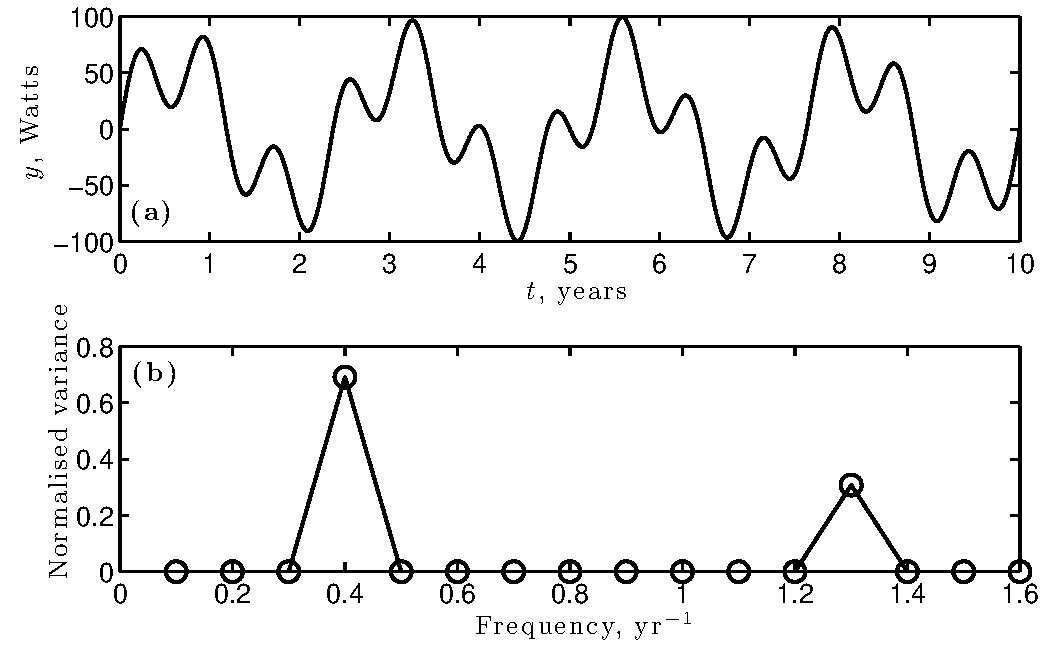
\includegraphics[width=5in]{../figs/L15/SeriesAndSpectrum_1}
  \caption{\textbf{(a)} Synthetic time-series and \textbf{(b)}
    normalised variance (power) spectrum.}
  \label{fig:synthseries}
\end{figure}

Now we analyse the time-series, noting that we should first strip off
the last data-point so that our series is periodic and has an odd number
of entries:
\Minput{y = y(1:end-1);}
\Minput{F = dfs(y);}

Lastly, we produce our variance spectrum, calculating the frequency
values that go on the $x$-axis:
\Minput{N = length(y);}
\Minput{k = 1:(N-1)/2;}
\Minput{freq = k/T;}
\Minput{plot(freq(1:16),F.power(1:16),'-ok'); \% Just plot first 16}
\Minput{xlabel('Frequency, 1/year'); ylabel('Normalised variance');}

A plot of the time-series and frequency spectrum are shown in
\autoref{fig:synthseries}.

\begin{figure}[bt]
  \centering
  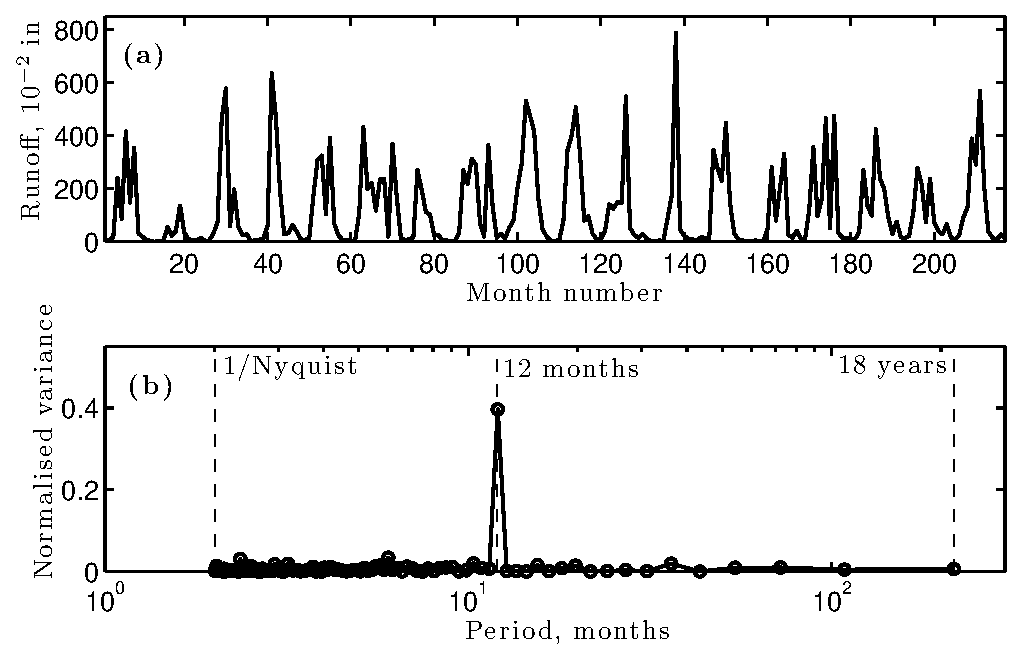
\includegraphics[width=5in]{../figs/L15/SeriesAndSpectrum_2}
  \caption{\textbf{(a)} Observed runoff at Cave Creek, and
    \textbf{(b)} normalised variance (power) spectrum. The shortest
    period, the 12-month, and the longest period oscillations are
    labelled. }
  \label{fig:runoffseries}
\end{figure}

As a second example, let's work with some real data: an 18-year record
of total monthly runoff of Cave Creek, in Kentucky,
France\footnote{Actually, there are 18 years plus 1 month of data in
  this series.  Why the extra month? Download the data from
  \url{http://www.earth.ox.ac.uk/~richardk/teaching/DTP/fourier/CaveCreekData.txt}}.
The data are given in hundredths of an inch.
\autoref{fig:runoffseries}a is a plot of the time-series.  Over the 18
years of recordings, there are about 18 peaks; this suggests that the
runoff peak occurs annually, which makes sense.  Let's analyse the
data.

Assuming that the data has been loaded and the time-series vector is
called \texttt{runoff},
\Minput{N = length(runoff);~\% check that N is odd!}
\Minput{F = dfs(runoff);}
\Minput{T = 18*12+1;~~~~~~~~\% total duration, months}
\Minput{k = 1:(N-1)/2;~~~~~~\% harmonic number}
\Minput{per = T./k;~~~~~~~~~\% periods}
\Minput{semilogx(per,F.power,'-ok','LineWidth',1.5,'MarkerSize',5);}
\Minput{xlabel('Period, months'); ylabel('Normalised variance');}\\[1mm]
The resulting plot is shown in \autoref{fig:runoffseries}b.  Note that
in this case, we have plotted the normalised variance against the
\textit{period} of oscillation, rather than the frequency.  This
sometimes makes the graph easier to understand.  Just as we
anticipated, most of the power in the signal is in the 12-month
oscillation. 

\subsection{What is a spectrum?}

In trying to get a feeling for the meaning of a spectrum, it is
helpful to consider what happens to visible light as it goes through a
prism. \autoref{fig:prism} shows electromagnetic waves of white light
incident on a prism from the right.  The prism bends different
frequencies of electromagnetic oscillations to different extents, and
hence separates the white light into its components.  The intensity of
each band of colour in the spectrum corresponds to the contribution of
that frequency to the white light.  This is a good analogy for the
variance or power spectrum: a plot of the contribution to the total
signal as a function of frequency (or period, or harmonic number,
etc).

\begin{SCfigure}[1][bh]
  \centering
  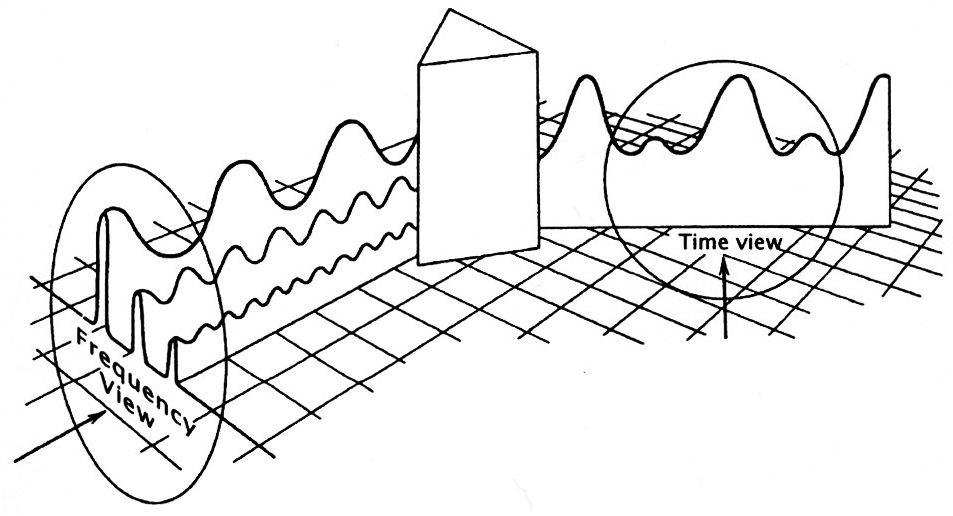
\includegraphics[width=4in]{../figs/L16/FourierPrism}
  \caption{(Fig.~4.75 from \textbf{DA}). A prism acts as a frequency
    analyser, transforming the incident white light (time or spatial
    view) into its constituent spectrum of colours (frequency
    view). The intensity of each colour in the frequency view is
    analogous to the amplitude in a variance (power) spectrum.
    \vspace{5mm}}
  \label{fig:prism}
\end{SCfigure}

%%%%%%%%%%%%%%%%%%%%%%%%%%%%%%%%%%%%%%%%%%%%%%%%%%%%%%%%%%

\section{Discrete Fourier Series and FFTs}
\label{sec:intro_timeseries}

\paragraph{In this section} we'll encounter a special consideration
when calculating the discrete Fourier series for time-series data that
have a long-term trend. We'll then introduce the concept of a Fourier
transform and learn about the built-in functionality of \Mlab for
Fourier analysis.

\subsection{Detrending} 

So far, we've applied Fourier analysis to
time-series that are \textit{stationary}: they have a mean that is
roughly constant with time, if one averages over the observed
oscillations. This is not true of all time-series.  Some have a
\textit{trend}, as well as periodic and random components.  Let's
consider an example of a synthetic time-series.
\Minput{T = 100;  \% years}
\Minput{N = 1001; \% data points}
\Minput{t = linspace(0,T,N+1);}
\Minput{y = 2*cos(2*pi*t*5/T)+sin(2*pi*t*12/T)+8*t/T+0.4*randn(size(t));}\\[1mm]
Our time-series \texttt{y}, shown in \autoref{fig:trendseries}a, 
has four components:
\begin{enumerate}
\item \texttt{2*cos(2*pi*t*5/T)} is a cosine component with amplitude 2 and
  period \texttt{T/5} = 20 years.  We therefore expect $\alpha_5=2$.
\item \texttt{sin(2*pi*t*12/T)} is a sine component with unit amplitude
  and period \texttt{100/12}. We expect $\beta_{12}=1$.
\item \texttt{8*t/T} is the trend in the dataset.  The time-series has
  a mean slope of \texttt{8/100}.
\item \texttt{0.4*randn(size(t))} is a normally-distributed random
  (noise) component with amplitude 0.4 (see \texttt{help randn} for
  details). 
\end{enumerate}

\begin{SCfigure}[1][tb]
  \centering
  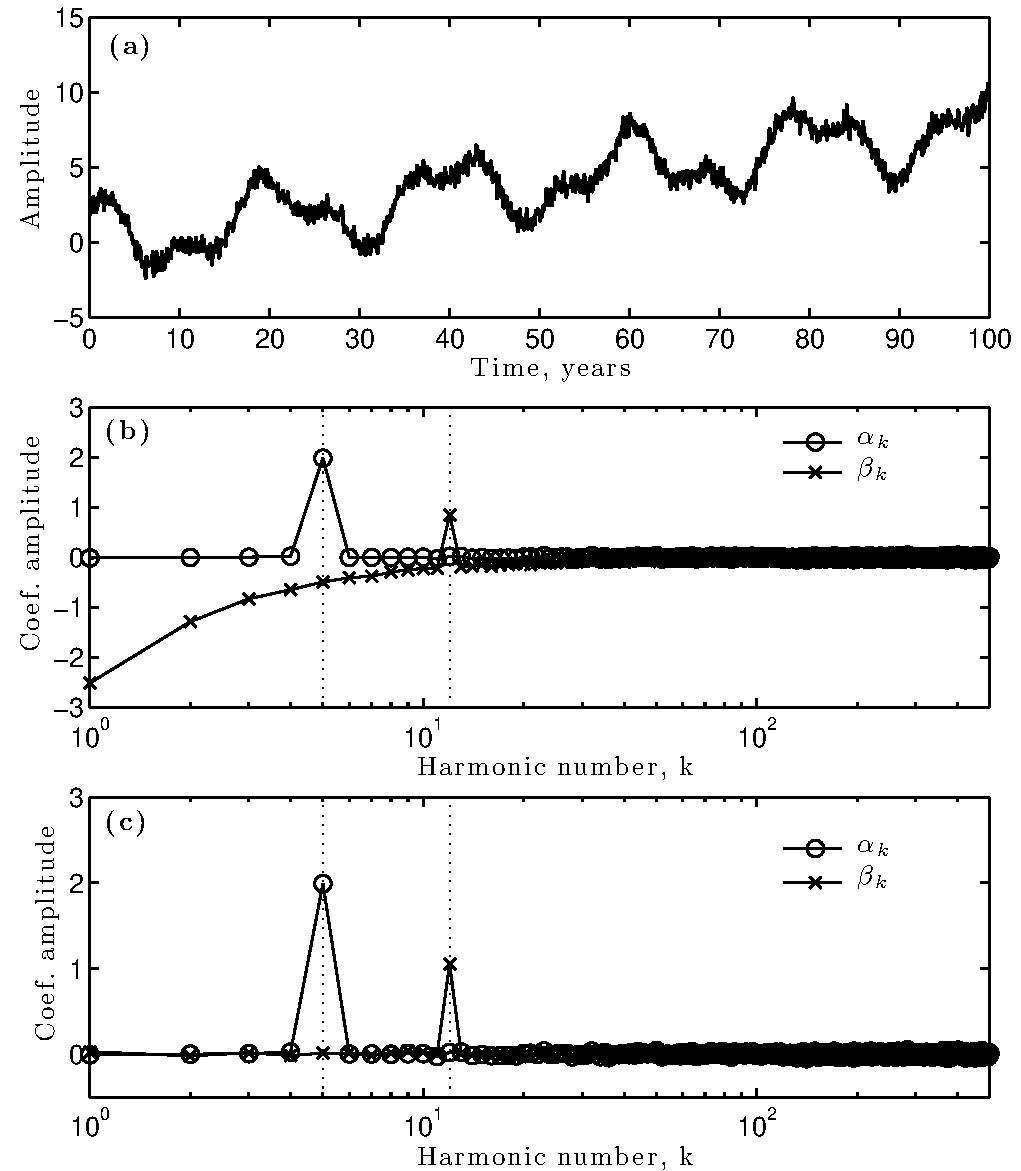
\includegraphics[width=4.5in]{../figs/L16/TimeSerWithTrend}
  \caption{\textbf{(a)} Synthetic time-series with two periodic
    components, a trend, and a random component. \textbf{(b)}
    Amplitude spectrum from the discrete Fourier series of the raw
    time-series, showing $\alpha_k$ (circles) and $\beta_k$,
    (crosses). Harmonic numbers 5 and 12 are marked with vertical
    dotted lines. \textbf{(c)} Amplitude spectrum of the detrended
    time-series.\vspace{1cm}}
  \label{fig:trendseries}
\end{SCfigure}

We then calculate and plot the discrete Fourier series,
\Minput{F = dfs(y(1:end-1));}
\Minput{k = [1:(N-1)/2];}
\Minput{semilogx(k,F.alpha,'-ok'); hold on;}
\Minput{semilogx(k,F.beta,'-xk');}
\Minput{plot([5 5],[-3 3],':k',[12 12],[-3 3],':k'); hold off;}
\Minput{xlabel('Harmonic number'); ylabel('Coef.~amplitude');}\\[1mm]
This amplitude spectrum is shown in \autoref{fig:trendseries}b. Note
that the values of of $\alpha_k$ are as expected: close to zero with a
spike at $k=5$ to about 2 (the random noise causes slight variations
from zero).  The values of $\beta_k$ are not as expected, however.
Although we see the expected spike at $k=12$, the values are below
zero for smaller values of $k$.  This downward curve is a consequence
of the trend in the time-series; \textit{remember that to compute the
  discrete Fourier series, we assumed that the time-series is
  periodic}.  The trend pollutes the Fourier coefficients with
deviations from zero that are unrelated to oscillations in the Fourier
series. To avoid this problem, it is often necessary to
\textit{detrend} a time-series before analysing.  This means
determining the linear (or non-linear) trend of the data-series and
subtracting it from the raw data.

Let's detrend the data and try the Fourier analysis again.  In this
case, we know the linear trend in the data, so we can subtract it off
directly; normally, if you had a measured time-series, you'd need to
regress the series to find the best-fitting trend, and then subtract
that trend off.
\Minput{ydt = y - 8/T*t;}
\Minput{Fdt = dfs(ydt(1:end-1));}
\Minput{semilogx(k,Fdt.alpha,'-ok'); hold on;}
\Minput{semilogx(k,Fdt.beta,'-xk');}\\[1mm]
A plot of the coefficients of the discrete Fourier series of the
detrended time-series is shown in \autoref{fig:trendseries}c. Note
that the spurious depression of the sine coefficients has been
eliminated. 

\subsubsection{Removing nonlinear trends}

\begin{SCfigure}[1][hb]
  \centering
  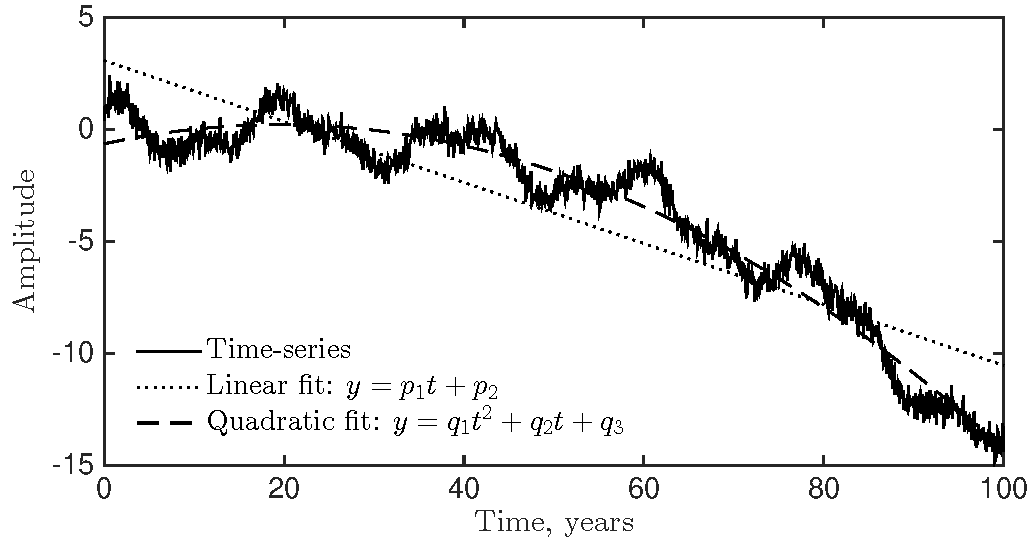
\includegraphics[width=4.5in]{../figs/L16/QuadDetrend}
  \caption{A synthetic time-series with a nonlinear trend.  Note that
    the dotted line, which is the best fit for a first order
    polynomial, is a still a poor fit to the trend in the data, while
    the second order (quadratic) polynomial captures the trend
    well. \vspace{0.1cm}}
  \label{fig:quad}
\end{SCfigure}

Trends in time-series are not always linear.  Sometimes they have
obvious curvature, which cannot be accommodated by a best fitting
straight line.  Let's consider another synthetic time-series as an
example, as shown in \autoref{fig:quad}.  In this figure, the
best-fitting straight line clearly does not fit the data. However, the
best-fitting quadratic polynomial fits the data very well.  Both of
these lines were calculated using the \Mlab built-in function
\texttt{polyfit}. Here's how it works (assuming that we have a vector of
times \texttt{t} and a vector of data \texttt{y}, both of the same length):
\Minput{p = polyfit(t,y,1)}\\
where \texttt{1} indicates that we want to use a polynomial of
degree one, i.e.~$y=p_1t + p_2$, where $p_1$ and $p_2$ are constants
to be determined by \Mlab.  This function returns
\begin{verbatim}
      p = 
           -0.1359    3.0590
\end{verbatim}
which are the constants $p_1$ and $p_2$ of our linear (degree one)
polynomial.  We can use the same function to obtain the coefficients
of a best-fitting quadratic polynomial,
\begin{verbatim}
      >> q = polyfit(t,y,2)

      q =
           -0.0022    0.0840   -0.6033
\end{verbatim}
\Mlab computes the coefficients of these polynomials using a linear
least squared error algorithm, that is very similar to what you
studied at the end of last term.  It is very easy to make a plot like
the one in \autoref{fig:quad}:
\Minput{plot(t, y, '-k'); hold on;}
\Minput{plot(t, p(1)*t + p(2), ':k');}
\Minput{plot(t, q(1)*t.\^{}2 + q(2)*t + q(3), '--k'); hold off;}\\
Wonderful!  We could easily plot a detrended version of the data by saying
\Minput{plot(t, y - (q(1)*t.\^{}2 + q(2)*t + q(3)), '-k');}

What order of polynomial should you use?  The higher the order, the
closer the fit to the time-series.  But higher order polynomials also
have more ``wiggles,'' and it is exactly these wiggles that spectral
analysis seeks to quantify.  So a good policy is to use lowest order
polynomial that effectively captures the trend without capturing the
wiggles that you are interested in.  This is somewhat subjective!

\subsection{The Fourier transform and its discrete version}

Fourier transforms are closely related to Fourier series, but take a
mathematical approach that is more complicated in order to achieve
greater generality of usage. For example, Fourier transforms can be
used on non-periodic functions.  You can think of a non-periodic
function as a periodic function where the period has gone to
infinity.  In this limit, the summation over frequencies that appears
in \autoref{eq:fourierseries} becomes an integral, and we have
\begin{subequations}
  \label{eq:fouriertransform}
  \begin{align}
    \label{eq:reverseft}
    {f}(t) &=
    \frac{1}{2\pi}\int_{-\infty}^{+\infty}\text{e}^{i\omega
      t}{F}(\omega)\,\infd \omega,\\
    \label{eq:forwardft}
    {F}(\omega) &= \;\;\;\;\;\;\int_{-\infty}^{+\infty}\text{e}^{-i\omega
      t}{f}(t)\,\infd t, 
  \end{align}
\end{subequations}
where $F(\omega)$ is the Fourier transform of the function
$f(t)$. \autoref{eq:reverseft} reconstructs the function in the
time-domain from its Fourier transform, and hence corresponds with
\autoref{eq:fourierseries}, while \autoref{eq:forwardft} corresponds
to recipe for calculating the Fourier series coefficients,
\autoref{eq:coefrecipe}.

The mathematics of the Fourier transform is beyond the scope of this
course, but we can make a couple of remarks about
\autoref{eq:fouriertransform}.
\begin{itemize}
\item The Fourier transform replaces the integer harmonic number $k$
  with a continuous angular frequency $\omega$.
\item It replaces the pair of coefficients $\alpha_k$ and $\beta_k$
  with a complex function $F$. Recalling Euler's formula
  \begin{displaymath}
    \text{e}^{i\theta} = \cos\theta + i\sin\theta,
  \end{displaymath}
  we can see that the real part of $F$ corresponds to the coefficients
  of the cosine terms $\alpha$, while the imaginary part of $F$
  corresponds to the coefficients of the sine terms $\beta$.
\end{itemize}
Like the Fourier series, the Fourier transform can be applied to
analytical functions, not to time-series data.  To analyse discrete
time-series data, we need the discrete version of the Fourier series.

The discrete Fourier transform is the method of spectral analysis that
is preferred by most scientists, and it is the method that is built
into \Mlab.  It is therefore a goal of this course to make it familiar
to you on a practical level.

Suppose that you have a time-series $\bv{y}$ composed of $N$
observations, equally spaced in time and covering a total time $T$. To
analyse this we use a discrete version of \autoref{eq:forwardft}, we
convert the integral back into a sum to give
\begin{equation}
  \label{eq:discretefouriertrans}
  Y_k = \sum_{n=1}^N y_n\,\exp\left[-2\pi i
    (k-1)\frac{n-1}{N}\right],\;\;\;\; 1\le k \le N,
\end{equation}
where $n$ is an index of the observations in the time-series and $k$
is the integer harmonic number.  $Y_k$ are the entries in a vector of
complex numbers, where
\begin{align}
  \alpha_k &= \text{Real}(Y_k), \\
  \beta_k &= -\text{Imag}(Y_k).
\end{align}
You may wonder why $k$ goes from 1 to $N$ in
\autoref{eq:discretefouriertrans}, whereas in the discrete Fourier series
it went from 1 to the Nyquist frequency at $(N-1)/2$.  The harmonics
for $k$ greater than the Nyquist frequency are \textit{image
  frequencies}, and are actually duplicates of the regular set.  For
technical reasons, it is easier to compute this complete series and
discard the image frequencies; this is what \Mlab does.

\subsection{Using \Mlab's \texttt{fft} function}

It should come as no surprise that \Mlab has a built-in function to do
spectral analysis.  This function is called \texttt{fft}, which is an
abbreviation of ``Fast Fourier transform''. \texttt{fft} is a rather
complicated tool.  It performs a discrete Fourier transform as
described in the previous section, and returns a set of complex
coefficients that has the same length as the input time-series.  For
example \Minput{y = rand([1 100]);} \Minput{Y = fft(y);}
\Matlab{length(Y)}{ans}{100} More details about \texttt{fft} can be
obtained using \texttt{help}.

% par explaining the output of fft & fftshift.

What we seek here is a means to convert the output of \texttt{fft}
into something we understand: the output of \texttt{dfs}.  The
following \Mlab function achieves this\footnote{For a more thorough
  discussion, see
  \url{http://www.mathworks.com/support/tech-notes/1700/1702.html}.},
and demonstrates the relationship between \Mlab's \texttt{fft} and the
discrete Fourier series.

\verbatiminput{../figs/L16/dft.m}

Let's examine this function in terms of its three steps:
\begin{enumerate}
\item Apply \texttt{fft} to the data-series.  The \texttt{fft}
  function works regardless of the length (even or odd) of the input
  time-series \texttt{y}.
\item Extract only the \texttt{fft} coefficients that are unique.
  This means discarding the second half of the entries, which
  correspond to the image frequencies. Since \texttt{N} can be even or
  odd, we must use rounding to ensure that \texttt{Nu} is an integer;
  \texttt{ceil} rounds upward, which is correct for any value of
  \texttt{N}. We then restrict \texttt{Y} to the desired set of
  values.
\item Scale the results appropriately, so that they are independent of
  time-series length, and consistent with the results of \texttt{dfs}.
\end{enumerate}

\subsection{Spectra, waves, and the Earth}

Fourier analysis decomposes a signal into a set of oscillations, and
represents the relative contributions of those oscillations on a
spectrum plot. One of the most commonly encountered oscillations is a
\textit{vibration}: the oscillatory physical motion of a
material. Because vibrations are inherently periodic, they are
amenable to Fourier analysis.

\begin{SCfigure}[1][tb]
  \centering
  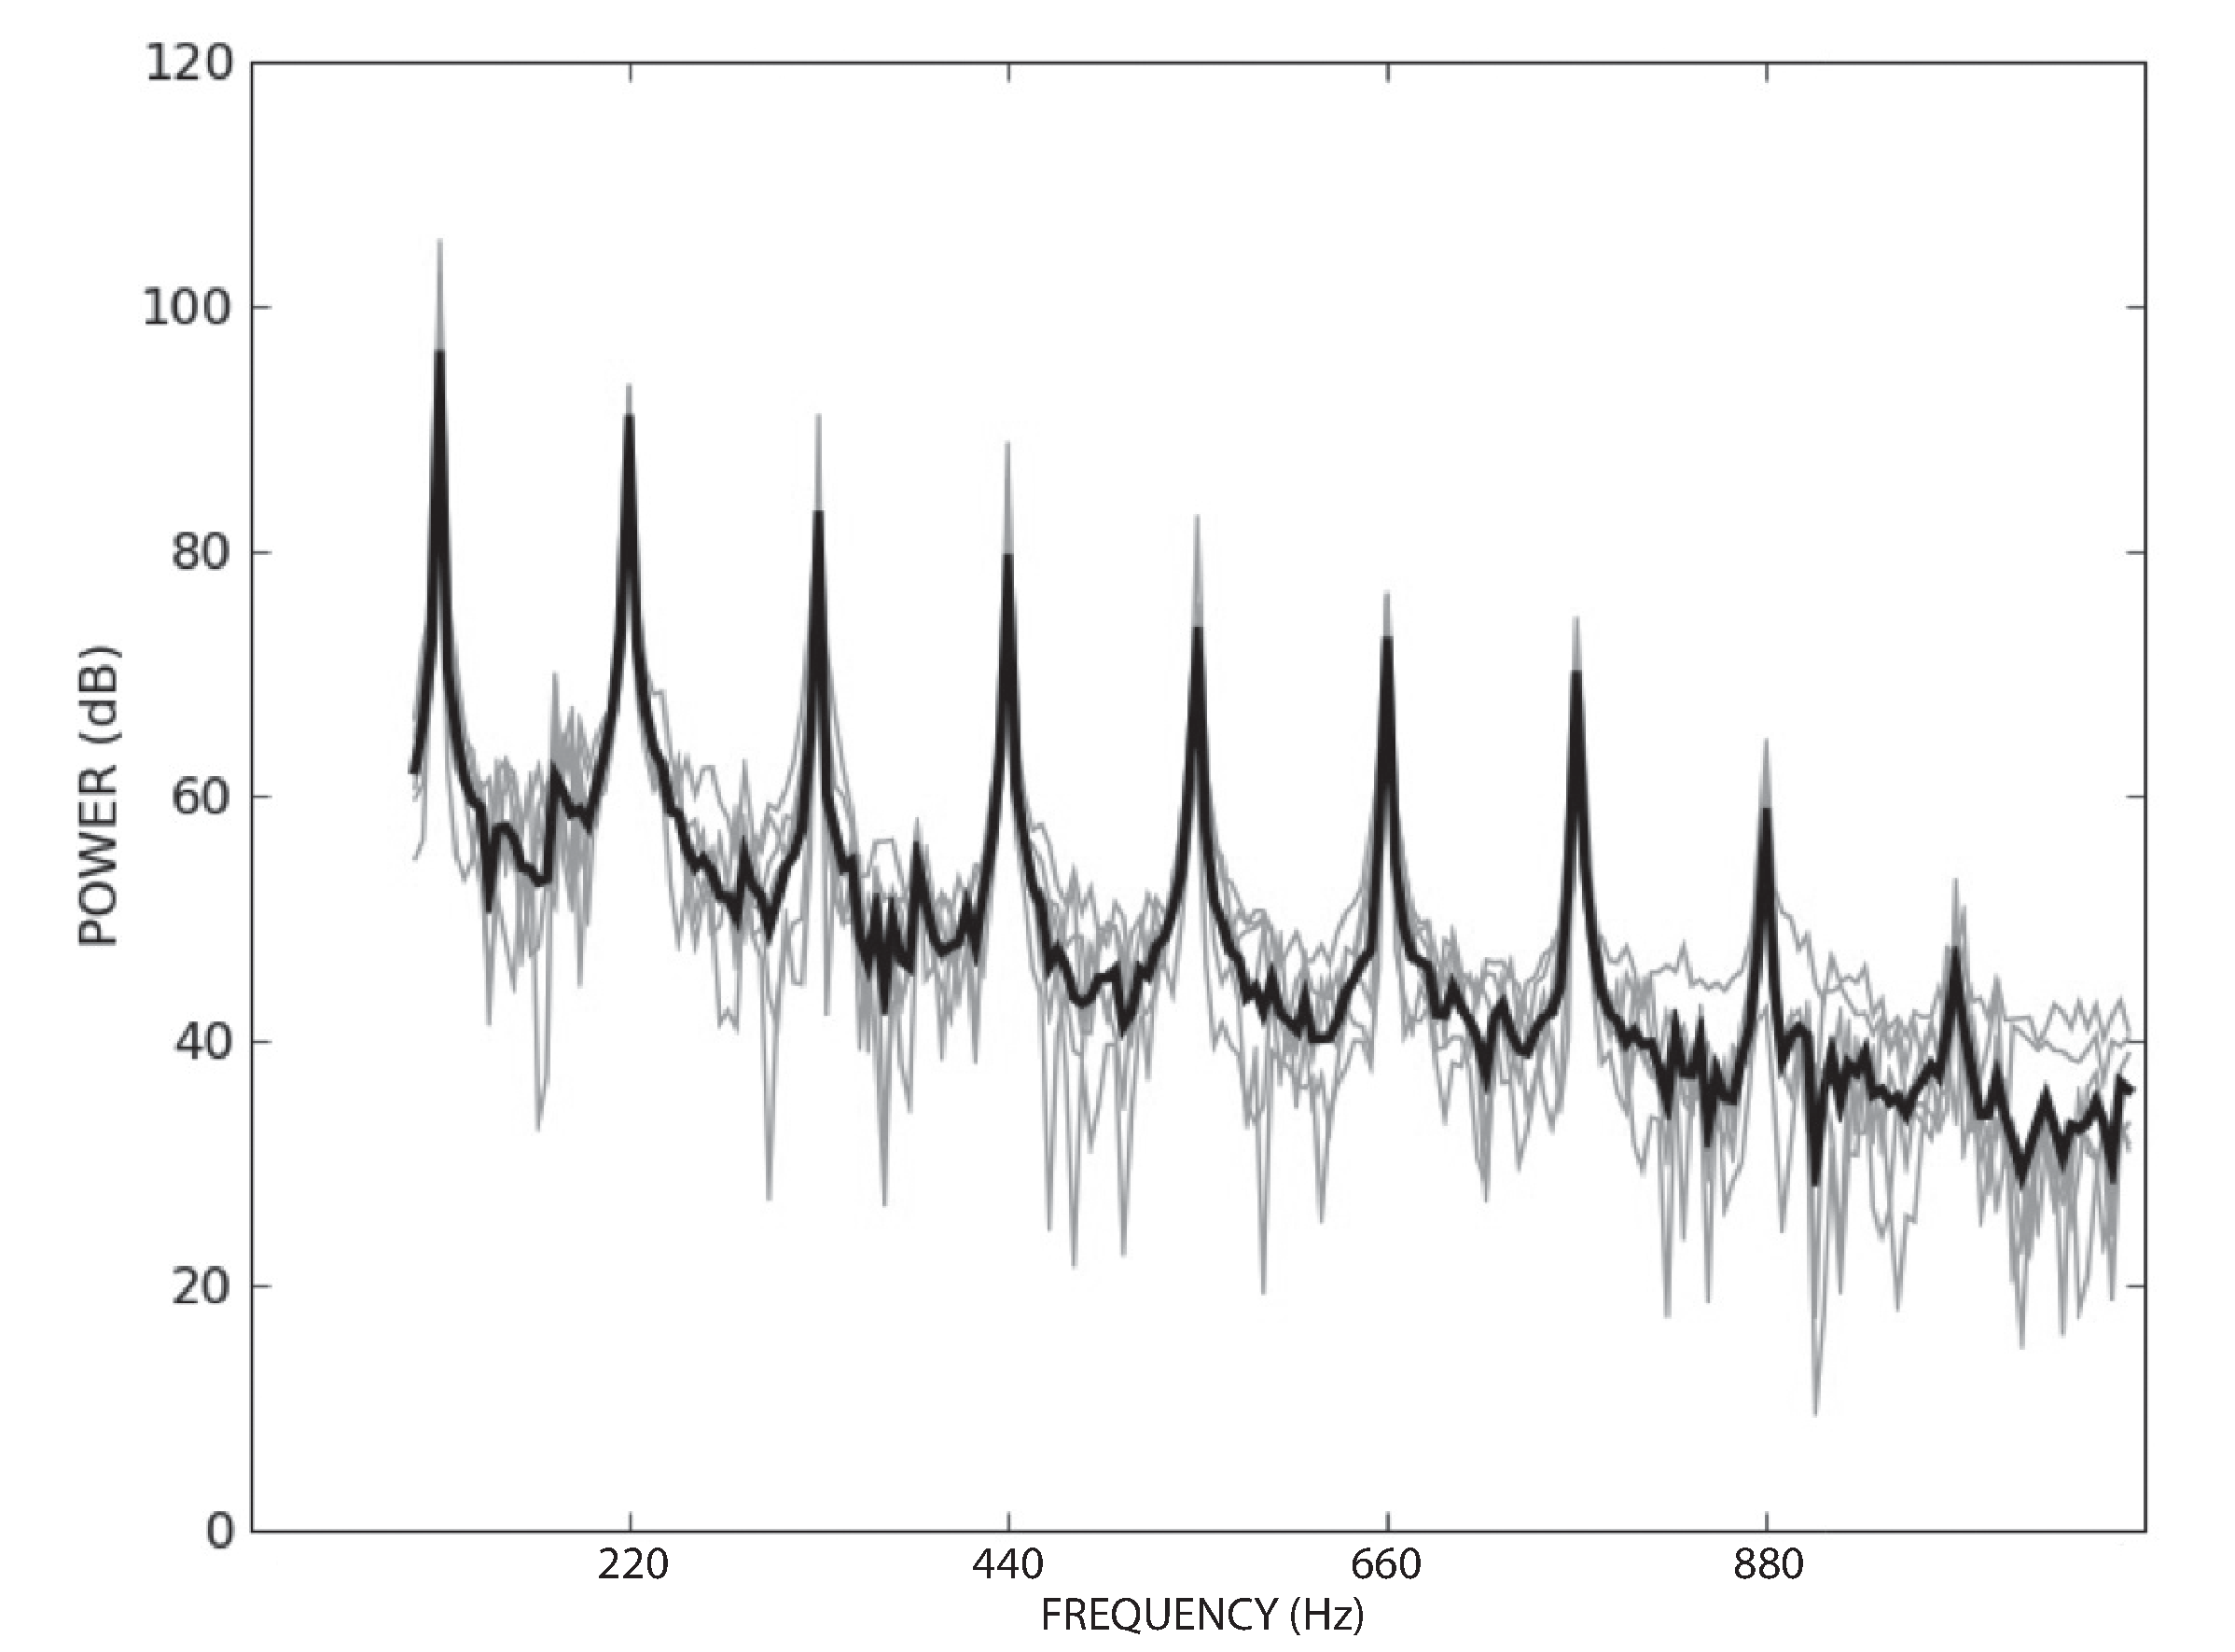
\includegraphics[width=4.5in]{../figs/L16/GuitarOvertones}
  \caption{Variance spectrum of the sound produced by a plucked guitar
    string. Grey lines are individual instances; heavy black line is
    the average of six instances. Adapted from report by
    M.~Owen.\vspace{1cm}}
  \label{fig:guitar}
\end{SCfigure}

Consider the vibration of a guitar string.  The averaged Fourier
spectrum of a plucked string is shown in \autoref{fig:guitar}. Note
the regular peaks in power at multiples of the \textit{fundamental
  frequency}, which in this case is 110 Hz.  The fundamental frequency
has the most power (i.e.~it is the loudest), but the vibrations at
higher frequency contribute substantially to the sound, while
vibrations at frequencies between the peaks are relatively quiet.
These regular peaks at frequencies that are multiples of the
fundamental frequency are known as \textit{overtones}, and their
contribution is what gives a musical instrument its unique sound.

\begin{figure}[ht]
  \centering
  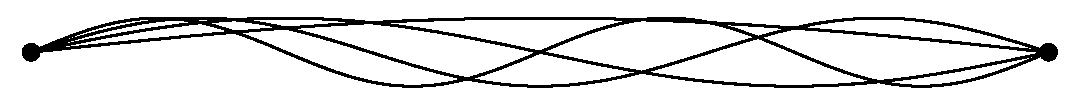
\includegraphics[width=\textwidth]{../figs/L16/NormalModes.pdf}
  \caption{Normal modes of a vibrating string that is fixed at its
    ends. The fundamental mode has the longest wavelength, equal to
    twice the length of the string, and can be written as $y(x,t) =
    A(t)\sin\left(\pi x/L\right)$, where $L$ is the length of the
    string. The others are described by $y(x,t) = A(t)\sin\left(n\pi
      x/L\right)$ for $n=2,3,...$}
  \label{fig:normalmodes}
\end{figure}

Where do overtones come from?  They are associated with a particular
set of oscillations that have a spatial structure that is unchanging
with time, and goes to zero at the fixed end-points. Hence they are
sometimes called \textit{standing waves}. Of course, since they are
vibrations, the displacement of the string must change with time; this
can be accommodated with a time-dependent amplitude
\begin{equation}
  \label{eq:string}
  y(x,t) = A(t)\sin\left(n\pi x/L\right) = A_0\sin(\omega_nt)
  \sin\left(n\pi x/L\right),
\end{equation}
where $A_0$ is a constant amplitude, $L$ is the length of the string,
and $n$ is an integer. Such oscillations are also known as the
\textit{normal modes} of the string. The wavenumber of each mode is
defined as
\begin{displaymath}
  \kappa_n = \frac{n\pi}{L};
\end{displaymath}
$n=1$ corresponds to the fundamental mode, and oscillations with $n>1$
are overtones.

As we will learn next term when we consider the physics of waves,
there is a physical relationship between the angular frequency of
oscillation for each normal mode $\omega_n$ and the mode number
$n$. This relationship is expressed mathematically as
\begin{equation}
  \label{eq:frequencies}
  \omega_n = c\kappa_n = \frac{cn\pi}{L},
\end{equation}
where $c$ is a constant, and a property of the string.  Examining the
spectrum shown in \autoref{fig:guitar}, we can identify the $n=2$ mode
with 220 Hz.  We then expect the fundamental mode at 110 Hz, and the
$n=4$ mode at 440 Hz.  The observations bear this out.

\begin{figure}[hb]
  \centering
  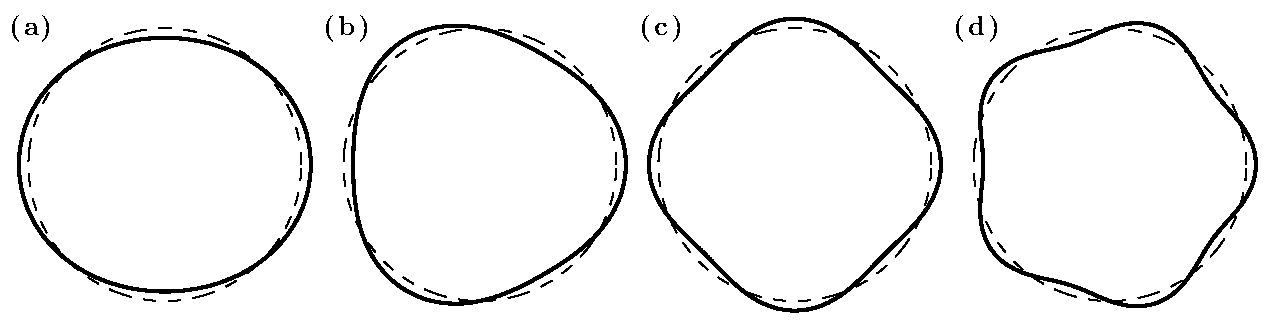
\includegraphics[width=\textwidth]{../figs/L16/HoopNormalModes}
  \caption{Four normal modes of a vibrating hoop. The dashed circle
    shows the undeformed hoop.\vspace{1cm}}
  \label{fig:hoop}
\end{figure}

Any finite vibrating object can possess a set of normal modes.
Consider, for example, a hoop as shown in \autoref{fig:hoop}.  This is
different from the string in that its ends are not fixed, but rather
it ``bites its own tail;'' hence the radial displacement of the hoop
must be periodic around the hoop with period $2\pi$.  With a little
imagination, you can generalise from a hoop to a spherical shell, or a
solid sphere, or even to the Earth!  Just as for the spectral analysis
of the sound produced by the vibrating guitar string, spectral
analysis of a carefully recorded seismogram reveals the so-called
\textit{free oscillations} of the Earth.  \autoref{fig:freeosc} is an
example of the spectrum of free oscillations recorded after the great
Sumatra-Andaman earthquake of December 2004.

\begin{figure}[ht]
  \centering
  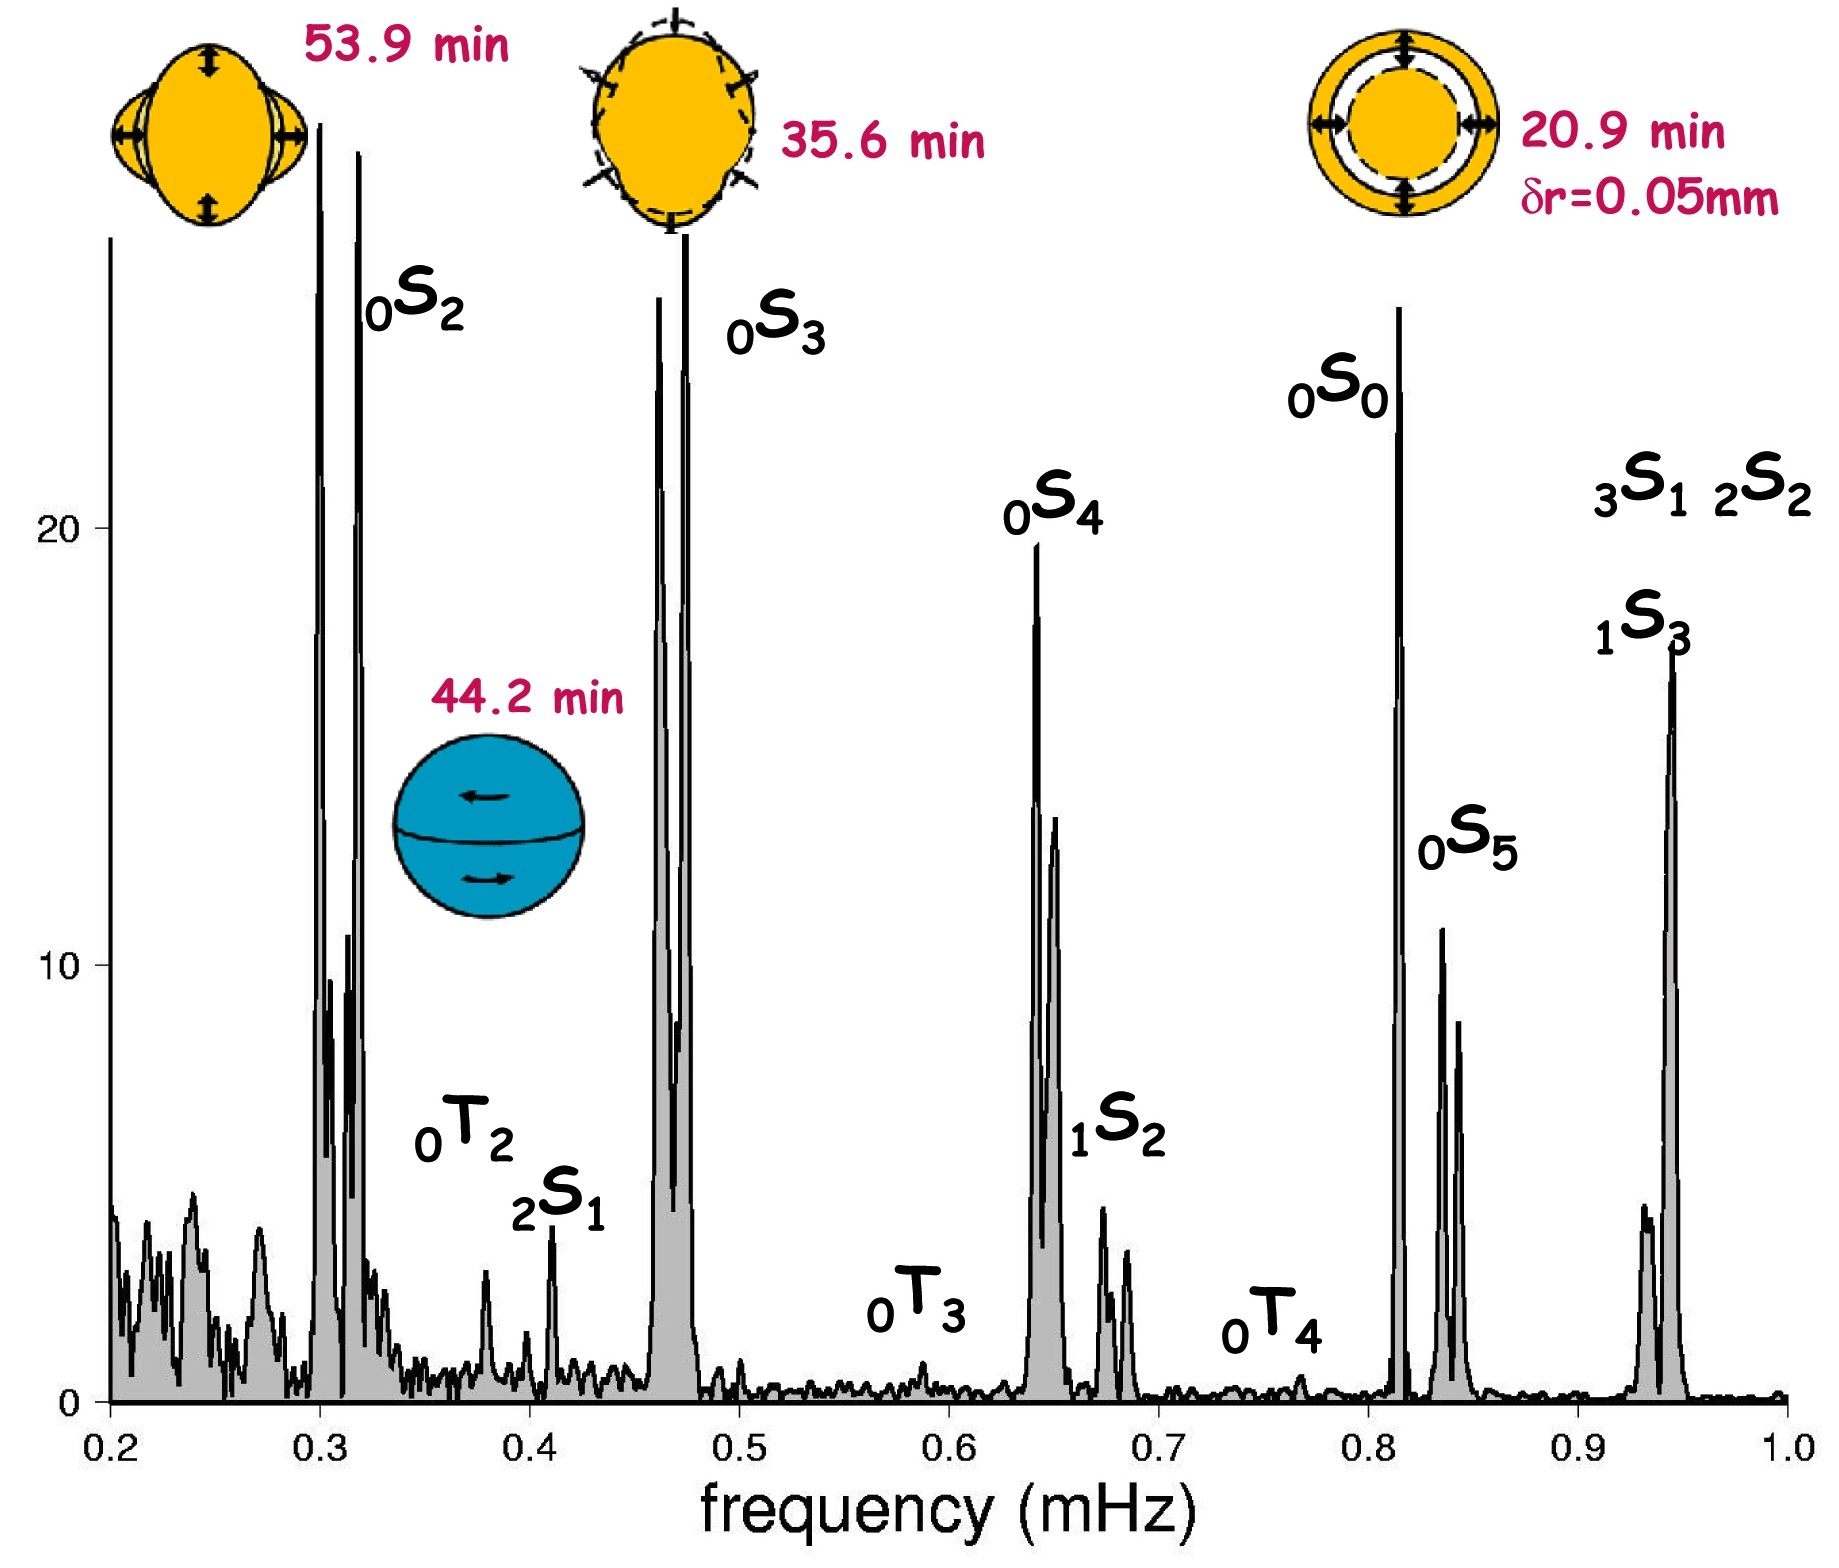
\includegraphics[width=\textwidth]{../figs/L16/NormalModeSpectrum}
  \caption{A spectrum of the normal modes of the Earth, also known as
    free oscillations. The modes labelled S are \textit{spheroidal
      modes}, where the displacement is toward or away from the centre
    of the Earth. The modes labelled T are \textit{toroidal modes},
    which involve displacements that are tangential to the surface of
    the Earth.  This spectrum was produced by a Fourier analysis of
    the free oscillations excited during the great Sumatra-Andaman
    earthquake of December 2004. (Figure credit Jeffrey Parks, Yale
    University).}
  \label{fig:freeosc}
\end{figure}

%%%%%%%%%%%%%%%%%%%%%%%%%%%%%%%%%%%%%%%%%%%%%%%%%%%%%%%%%%%%%%%%%%%

\section{Diffusion}
\label{sec:diffusion_2}

\paragraph{In this section} We'll derive the diffusion equation for
non-steady situations.  We'll then investigate how a spatially
oscillating temperature field changes with time, due to diffusion.
This will allow us to apply tools of Fourier analysis to create
mathematical models of diffusion.

\subsection{The time-dependent diffusion equation}

\begin{figure}[ht]
  \centering
  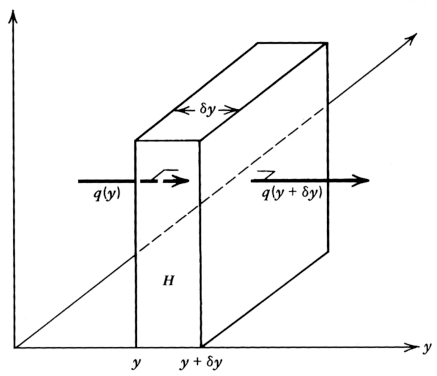
\includegraphics[height=2.5in]{../figs/L17/heatsourceslab}
  \caption{Heat flow into and out of a thin slab of rock. (source:
    \textbf{TS} chap.~4)}
  \label{fig:thinslab_again}
\end{figure}

Let's return to the trusty First law of thermodynamics, which tells us
that energy is conserved.  We'll again consider the case of a slab of
rock of thickness $\delta y$ as shown in \autoref{fig:thinslab_again}.
The First law reads
\begin{equation}
  \label{eq:firstlaw_time}
  \diff{U}{t} = \diff{Q}{t},
\end{equation}
which says that the rate of change of internal energy is equal to the
rate of net addition of heat.  Let's treat the right-hand side first.
The rate of net addition of heat can be broken down into its component
fluxes as
\begin{equation}
  \label{eq:heatfluxes}
  \diff{Q}{t} = q_\text{in} - q_{out} + q_\text{source}.
\end{equation}
In the last lecture, where we considered only steady-state, this sum
was equal to zero.  When we allow for changes in internal energy, the
left-hand side of \autoref{eq:firstlaw_time} becomes
\begin{equation}
  \label{eq:internalenergy}
  \diff{U}{t} = \rho c \diff{T}{t}\delta y,
\end{equation}
since the changes in internal energy comes only from changes in
temperature.  In this equation, $\rho$ is the density (kg-m$^{-3}$)
and $c$ is the specific heat capacity (J-kg$^{-1}$-K$^{-1}$).  Then
the units of \autoref{eq:internalenergy} are J-m$^{-2}$-sec$^{-1}$,
which is the same units as the various fluxes~$q$.

Equating the left-hand side and the right-hand side of the First law
we have
\begin{align}
  \label{eq:difn_deriv}
  \rho c \pdiff{T}{t}\delta y &= q_\text{in} - q_{out} + q_\text{source},\nonumber\\
                              &= \delta y \left(k\pdifftwo{T}{y} + \rho H\right),
\end{align}
and hence we have
\begin{displaymath}
  \rho c \pdiff{T}{t} = k\pdifftwo{T}{y} + \rho H.
\end{displaymath}
This is the time-dependent diffusion equation with a source term.  It
can also be written
\begin{equation}
  \label{eq:difneqn_source}
  \pdiff{T}{t} = \kappa\pdifftwo{T}{y} + \frac{H}{c},
\end{equation}
where $\kappa = k/(\rho c)$ is the \textit{thermal diffusivity}.  When
there is no radiogenic heat production, this equation becomes
\begin{equation}
  \label{eq:difneqn}
  \pdiff{T}{t} = \kappa\pdifftwo{T}{y}.
\end{equation}
Note the use of partial differentials in equations
\eqref{eq:difn_deriv}--\eqref{eq:difneqn}.  This is simply because we
now see that the temperature $T$ varies with both time $t$ and
position $y$.

\autoref{eq:difneqn} is the canonical diffusion equation in one
dimension, with constant thermal diffusivity. A few remarks about this
equation
\begin{itemize}
\item It is an equation for temperature $T$ as a function of time $t$
  and space $y$.  This can be represented mathematically as
  $T=T(t,y)$.
\item It is a \textit{linear} equation, because it does not involve
  nonlinear functions of $T$.
\item It is a \textit{first-order} partial differential equation in
  time, because it has a first derivative of $T$ with respect to
  $t$. To solve it we must therefore specify an \textit{initial
    condition} in the form of $T(0,y) = f(y)$, where $f(y)$ is some
  function of position only.
\item It is a \textit{second-order} partial differential equation in
  space, because it has a second derivative of $T$ with respect to
  $y$.  To solve it on a finite domain, we must therefore specify two
  boundary conditions.  For example, if the domain is $0\le y \le 1$,
  we could specify the boundary conditions
  \begin{subequations}
    \begin{align}
      T(t,0) &= 0,\\
      T(t,1) &= 12.
    \end{align}
  \end{subequations}
  Note that in the previous lecture, when we solved the steady-state
  diffusion equation, we also needed two boundary conditions.  That
  equation is also second-order in space.
\end{itemize}
The rest of the lecture will focus on methods of solving this
equation.

\subsection{Diffusion in an insulated rod of infinite length}

Let's begin solving the diffusion equation with a simple example.
We'll consider a perfectly insulated rod of infinite length.  Since
the rod is insulated, we can assume that temperature is only conducted
along the rod, in the $y$-direction. By giving the rod infinite
length, we avoid the neccessity to specify boundary conditions.  We
still need an initial condition, however.  For reasons that will
become clear later, let's choose a sinusoidal variation
\begin{equation}
  \label{eq:IC}
  T(0,y) = A\sin\left(\frac{2\pi}{\lambda}y\right),
\end{equation}
where $A$ is the amplitude of the variations and $\lambda$ is the
wavelength (note that when $y=\lambda$, the argument to the sine
function is $2\pi$, and hence we've gone through a full cycle). The
problem becomes the following: \textit{how does the initial
  distribution of temperature evolve with time?}  Another way of
stating this is \textit{given this initial condition, what is the
  distribution of temperature at time $t$?}

Our physical intuition tells us that heat should diffuse away from the
peaks in temperature and towards the troughs.  Our mathematical
intuition confirms this: at the temperature peaks,
$\partial^2 T/\partial y^2 < 0$; hence we have
$\partial T/\partial t < 0$ at the peaks.  At the troughs, the
situation is reversed, and the temperature should trend upwards.  So
we should expect the amplitude of the oscillation to decay away with
time.

With this expectation in mind, let's start with a clever guess.
Having solved linear equations in the past, we know that the solution
often takes the form $\expu{\alpha x}$, where $x$ is the independent
variable.  In this case, our independent variable is $t$, and so we
could try to solve the equation using the guess
\begin{equation}
  \label{eq:ansatz}
  T(t,y) = A\expu{\alpha t}\sin\left(\frac{2\pi}{\lambda}y\right).
\end{equation}

Is this the correct form of the solution?  A first check: when $t=0$,
\autoref{eq:ansatz} returns our initial condition from
\autoref{eq:IC}.  As a second check, let's plug \autoref{eq:ansatz} in
the diffusion equation \eqref{eq:difneqn} and see if it works:
\begin{align}
  \pdiff{T}{t} &= \kappa\pdifftwo{T}{y}, &&\text{Diffusion equation.}\nonumber\\
  \alpha A\expu{\alpha t}\sin\left(\frac{2\pi}{\lambda}y\right) &= 
                                                                  -\kappa\left(\frac{2\pi}{\lambda}\right)^2A\expu{\alpha
                                                                  t}\sin\left(\frac{2\pi}{\lambda}y\right),&&\text{By plugging in \eqref{eq:ansatz}.}\nonumber\\
  \label{eq:decayconst}
  \alpha &= -\kappa\left(\frac{2\pi}{\lambda}\right)^2.&&\text{By cancellation.}
\end{align}
So what we find is that as long as $\alpha$ takes the form given in
\autoref{eq:decayconst}, then our guess solution will work.  Hence we
can write the solution to our problem as
\begin{equation}
  \label{eq:soln1}
  T(t,y) = A\exp\left[-\left(\frac{2\pi}{\lambda}\right)^2\kappa\, t\right]
  \sin\left(\frac{2\pi}{\lambda}y\right).
\end{equation}
Try plugging this equation into \autoref{eq:difneqn} to verify that it
is, indeed a solution.

\begin{figure}[ht]
  \centering
  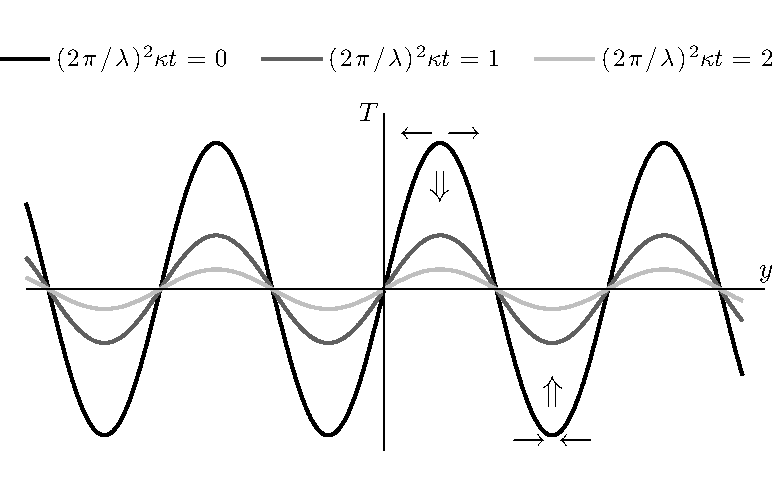
\includegraphics[height=2.5in]{../figs/L18/decayOscillations}
  \caption{A decaying, sinusoidal temperature variation. The black
    line is the initial condition; the lighter lines are solutions at
    subsequent times. The single-stemmed arrows indicate the
    directions of heat flow; the double-stemmed arrows indicate the
    change in temperature with time.}
  \label{fig:decayosc}
\end{figure}

What does our solution tell us about diffusion?  A few things are
evident:
\begin{itemize}
\item \autoref{eq:decayconst} tells us that the rate of decay is
  inversely proportional to the square of the wavelength.  Longer
  wavelength oscillations decay much slower than shorter wavelength
  oscillations.
\item \autoref{eq:decayconst} tells us that the rate of decay is
  proportional to the diffusivity.
\item \autoref{eq:soln1} tells us that diffusion does not cause a
  change in the wavelength of the oscillations, it only causes those
  oscillations to decay in amplitude.
\item This solution is only valid on an infinite domain.  We did not
  impose boundary conditions because there are no boundaries!
\end{itemize}

We can generalise this example to something more useful.  Let's
consider a more complex initial condition:
\begin{equation}
  \label{eq:IC3}
  T(0,y) = A_1\sin\left(\frac{2\pi}{\lambda_1}y\right) + 
  A_2\cos\left(\frac{2\pi}{\lambda_2}y\right) +
  A_3\sin\left(\frac{2\pi}{\lambda_3}y\right),
\end{equation}
where $A_i$ and $\lambda_i$ are the amplitude and wavelength of the
three different sinusoidal oscillations that compose our initial
distribution of temperature.  Since the governing equation
\eqref{eq:difneqn} is linear, we know that simpler solutions can be
added together to create more complex ones.  We can break our problem
up into three sub-problems, one for each term in \autoref{eq:IC3},
find their solutions, and then sum them.  Each sub-problem will have a
solution like \autoref{eq:soln1}, and hence we can immediately write
that the evolution of our initial condition \eqref{eq:IC3} is given by
\begin{align}
  \label{eq:soln3}
  T(t,y) = &A_1\exp\left[-l_1^2\kappa\,t\right] \sin\left(\frac{2\pi}{\lambda_1}y\right) + \nonumber\\
           &A_2\exp\left[-l_2^2\kappa\,t\right] \cos\left(\frac{2\pi}{\lambda_2}y\right) + \nonumber\\
           &A_3\exp\left[-l_3^2\kappa\,t\right]\sin\left(\frac{2\pi}{\lambda_3}y\right),
\end{align}
where $l_i = 2\pi/\lambda_i$ is the wavenumber.  We can see from this
solution that each of the initial oscillations decays at its own rate,
dependent on its wavelength (and on the thermal diffusivity),
independent of the others.  The solution is plotted for four different
times in \autoref{fig:threeDecays}.

\begin{figure}[ht]
  \centering
  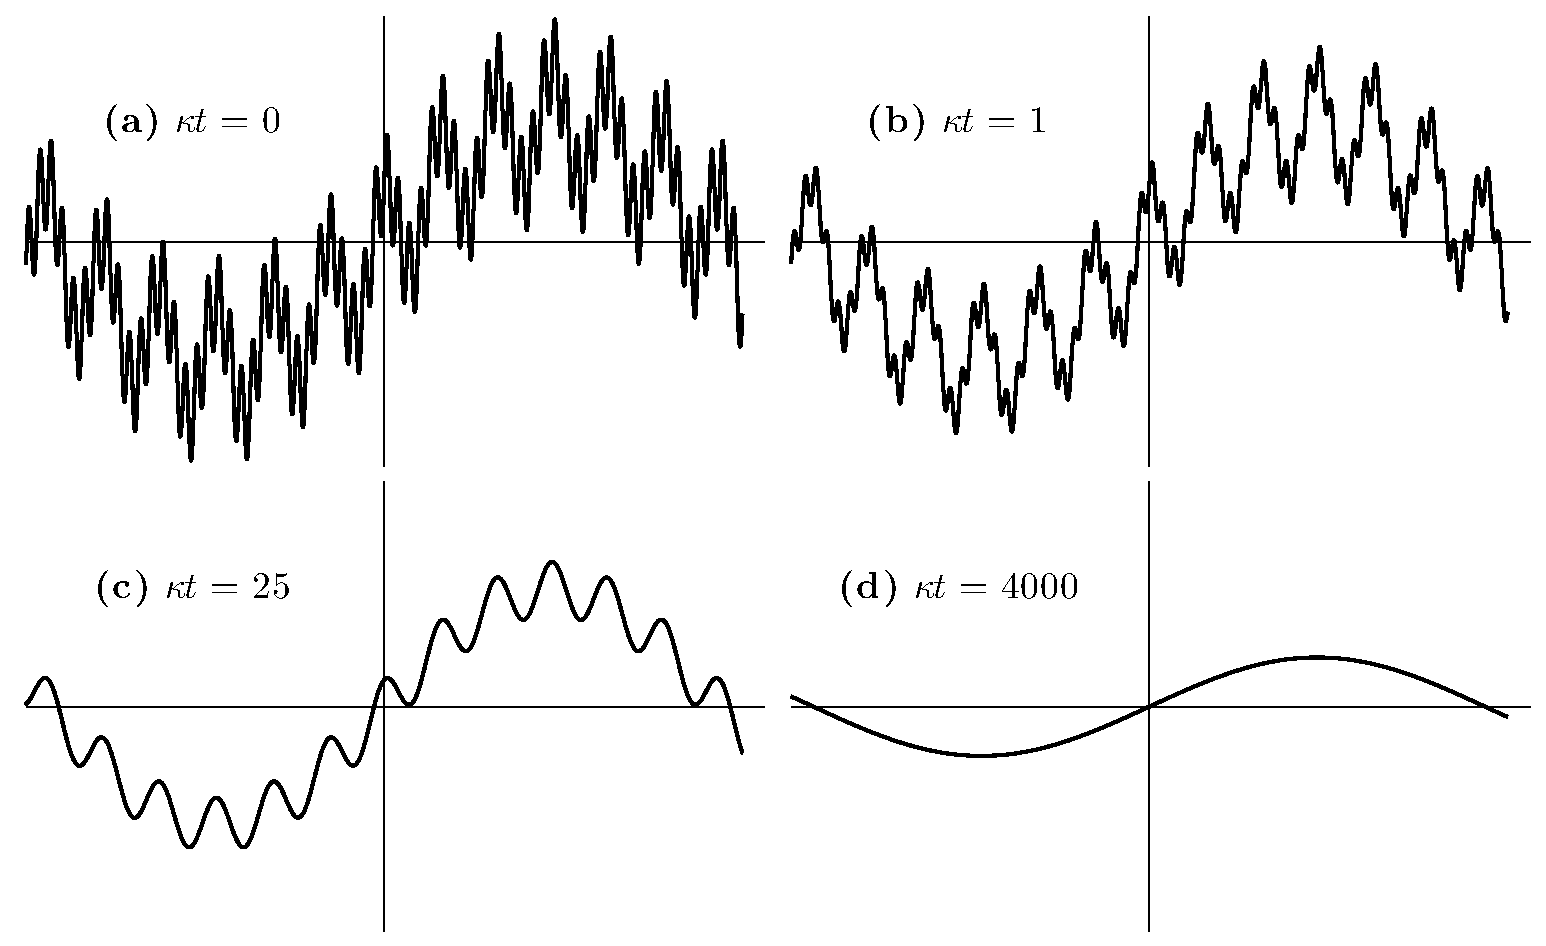
\includegraphics[height=3in]{../figs/L18/decayThreeOscillations}
  \caption{A plot of \autoref{eq:soln3} four different times. Note the
    three superimposed oscillations at $t=0$.  By $\kappa t=25$, the
    shortest wavelength oscillation has diffused away. By
    $\kappa t=4000$, the middle wavelength oscillations has diffused
    away, and the longest wavelength oscillation has decreased in
    amplitude.}
  \label{fig:threeDecays}
\end{figure}

More generally still, if our initial condition is the sum of
sinusoidal functions in space on an infinite domain, then we can we
can immediately write down a solution for their temporal evolution
under diffusion.  But we learned last term that \textit{we can write
  any periodic function in terms of the sum of sinusoidal functions!
  So we can apply this solution to any periodic function!}

For example, let's consider a situation where $T(0,y) = f(y)$, with
$f(y) = f(y+Y)$.  This means that we have an initial condition given
by some function $f$, which is periodic in the $y$-direction, with
some period $Y$.  We can use the Fourier series representation of our
initial condition
\begin{equation}
  \label{eq:ICfourier}
  T(0,y) = a_0 + \sum_{n=0}^\infty\left[a_n\sin(l_n y) + b_n\cos(l_n y)\right],
\end{equation}
where $l_n=2\pi/\lambda_n$ is the wavenumber corresponding to each
entry in the sum.  Given some function $f(y)$, coefficients $a_n$ and
$b_n$ can be obtained in the usual way, which we learned last term.

Without further ado, we can write down the time-evolution of the
initial condition as
\begin{equation}
  \label{eq:solnfourier}
  T(t,y) = a_0 + \sum_{n=0}^\infty
  \exp\left(-l_n^2\kappa t\right)\left[a_n\sin(l_n y) + 
    b_n\cos(l_n y)\right].
\end{equation}
This result is the exact solution of the diffusion equation
\eqref{eq:difneqn} for the initial condition given by $f(y)$.

\begin{figure}[ht]
  \centering
  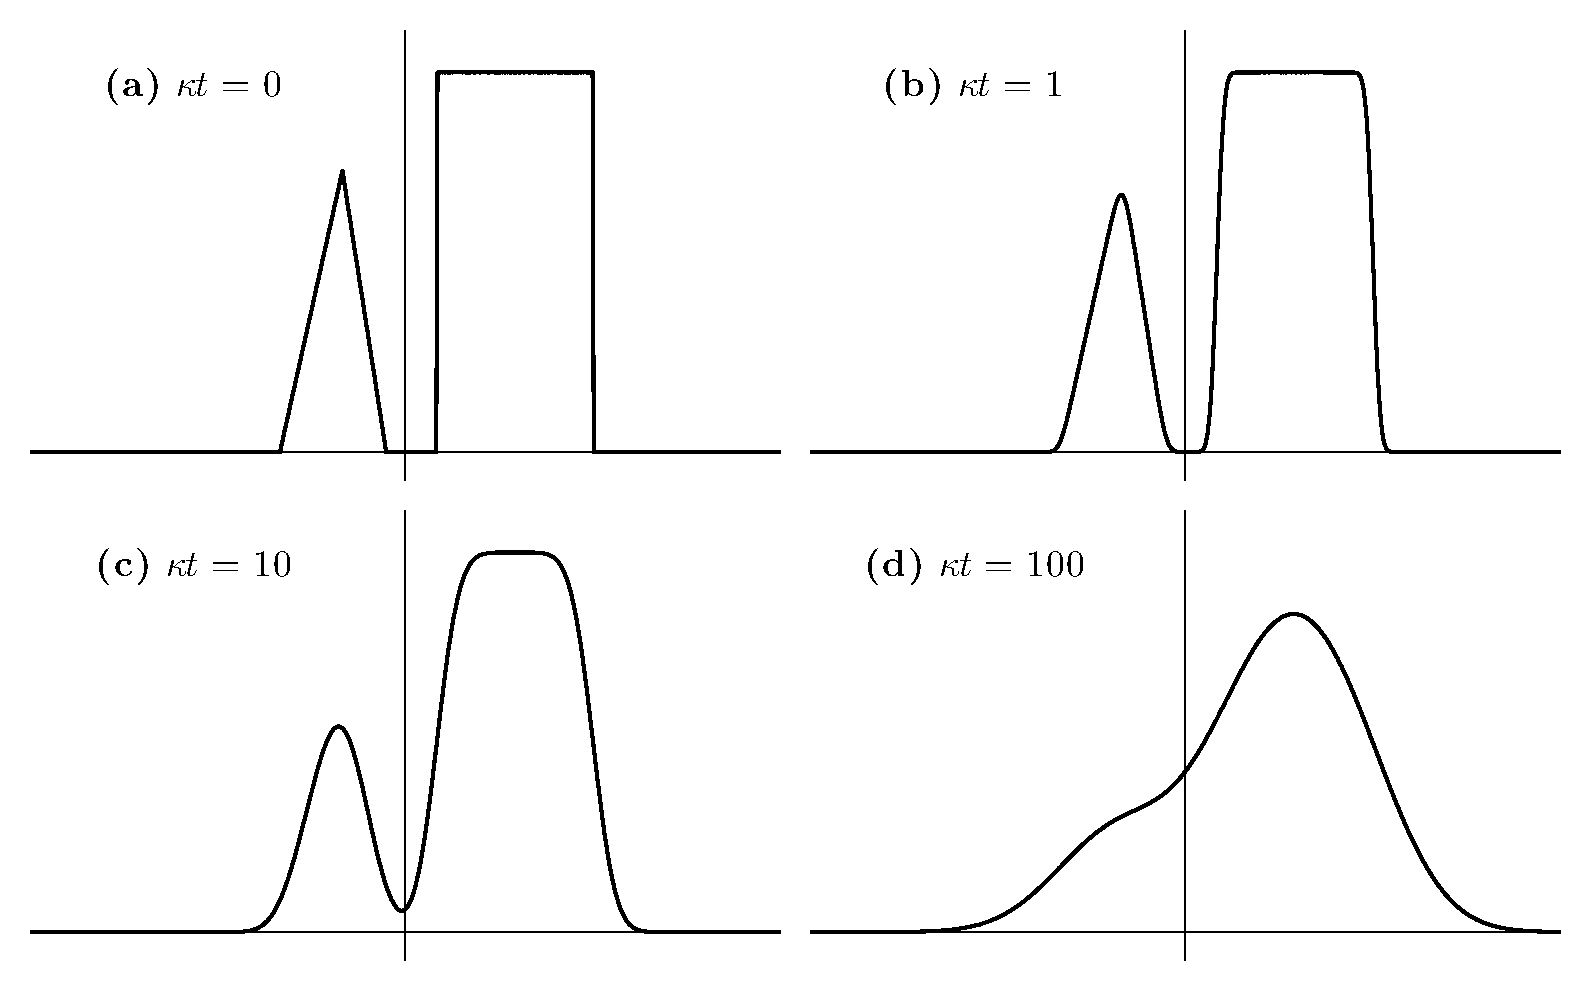
\includegraphics[height=2.5in]{../figs/L18/decayFourierOscillations}
  \caption{Romance, diffusion-style.}
  \label{fig:fourierDecay}
\end{figure}

Wow! Fantastic!  We can see this wonderful result in action in
\autoref{fig:fourierDecay}. Only one period of the function is shown,
but in fact this pattern repeats every $Y$ units from $-\infty$ to
$+\infty$.

\subsection{Mathematical lessons about diffusion}

We noted above that the rate of decay for a particular Fourier mode
under diffusion increases with the wave-number (or the inverse
wavelength) of the mode.  We can see from \autoref{fig:fourierDecay}
that because of this, diffusion acts as a \textit{smoother}, rounding
out sharp edges and blurring the initial condition. Since heat is
conserved, the integral of $T(t,y)$ must be constant for this model.

\subsection{Solving the infinite-rod diffusion problem with \Mlab}

In the previous section we learned that since each oscillatory
component of the initial condition decays independently of the others,
we can use the Fourier series of the initial condition as a means to
express the effect of diffusion over time.  How do we implement this
in \Mlab? We can build on the functions we developed last term.

We first need a function that, given an initial distribution of
temperature, and the time over which diffusion has taken place, will
return the temperature distribution at that time.  The steps to do
this are as follows
\begin{enumerate}
\item Compute the discrete Fourier series of the initial condition.
\item Determine the decay constant for each pair of Fourier
  coefficients $\alpha_n,\beta_n$.
\item Calculate and apply the amount of decay for each pair of Fourier
  modes.
\item Reconstruct and return the diffused temperature function from
  the decayed Fourier coefficients.
\end{enumerate}

Here's a function that does the trick:

\verbatiminput{../figs/L18/dfs_diffusion.m}

Using this function, we can solve for the evolution of an arbitrary
(periodic) distribution of initial temperature in the rod.  Let's try
an example in \Mlab.

%%%%%%%%%%%%%%%%%%%%%%%%%%%%%%%%%%%%%%%%%%%%%%%%%%%%%%%%%%%%%%%%%%%

\section{Waves}
\label{sec:waves_1}

\paragraph{In this section} we'll derive the partial differential
equation governing wave-motions of a stretched string. We'll find the
general solution to that equation, and show that it consists of a set
of arbitrary functions that move forward and backward with time.
We'll then consider the case of sinusoidal functions as waves, and
look at the standing wave-pattern generated by two identical
sinusoidal waves traveling in opposite directions.  We consider the
general solution for a finite segment of string, and use the Fourier
series (again!) as a tool to solve for the evolution of specific
initial conditions. We briefly consider the use of \Mlab to solve the
wave equation for a finite string.  

\subsection{The wave equation for an ideal streched string}

Consider a string with a mass of $\lambda_0$ per unit length and under
constant tension $\tau_0$, maintained by equal and opposite forces at
its ends.  In the absence of any waves, the string is straight; we'll
assume that it is infinitely long.  Define the $x$-axis as lying along
the unperturbed string. \EH{1.1}

We're interested in what happens when the string is locally displaced
from the $x$-axis, i.e.~it is plucked.  The tension in the string will
pull it back toward its equilibrium position on the axis.  However,
inertia will cause the string to overshoot this position.  Because of
the continuity of the string, the disturbance will spread, or
\textit{propagate}, away from its initial location with time.  We seek
an equation that governs this process.

To quantify this, we apply Newton's second law ($\sum_i F_i=ma$) to
any small element of the string of length $\Delta x$. We'll measure
the displacement from the $x$-axis with the variable $\eta$, and
assume that the string remains in the $x$-$y$ plane.  Then the
displacement is an unknown function of position and time,
$\eta=\eta(x,t)$.  We assume that $\eta$ is sufficiently small that
\begin{itemize}
\item The magnitude of the tension $\tau_0$ is constant, independent
  of $x$ and $t$.
\item The angle of inclination of the displaced string with respect to
  the $x$-axis at any point is small.
\item An element $\Delta x$ of the string can be considered to have
  moved only in the transverse direction as a result of a wave
  disturbance.
\end{itemize}
We also idealise by neglecting air drag on the string, the stiffness
of the string, and the effect of gravity.

\begin{figure}[ht]
  \centering
  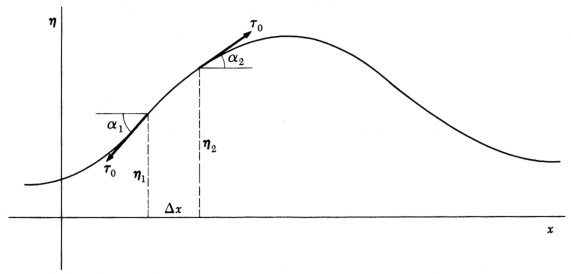
\includegraphics[height=2.5in]{../figs/L19/StringDiagram}
  \caption{Diagram of forces acting an element of string $\Delta x$
    due to the curvature of the string. (source: \textbf{EH} chap.~1)}
  \label{fig:stringbal}
\end{figure}

\autoref{fig:stringbal} shows a schematic diagram of a portion of the
string that has been displaced sideways from its equilibrium
position. A net force acts on an element of the string $\Delta x$
because, in general, the angles $\alpha_1$ and $\alpha_2$ (definied in
the figure) are not equal.  This unbalanced force has a component in
the $y$-direction given by $\tau_0(\sin\alpha_2 - \sin\alpha_1)$ and
in the $x$-direction $\tau_0(\cos\alpha_2 - \cos\alpha_1)$.  Recalling
that both angles are small, we can make a Taylor series expansion of
the sinusoidal functions
\begin{align}
  \sin \alpha &\approx \alpha + \mathcal{O}(\alpha^3)\approx\pdiff{\eta}{x},\nonumber\\
  \cos \alpha &\approx 1 - \mathcal{O}(\alpha^2)\approx 1.\nonumber
\end{align}
The second of these means that to leading order, we can neglect the
difference in the $x$-component of the force difference.  The first
means that we can replace $\sin\alpha_n$ with
$\partial\eta_n/\partial x$, where we have used the partial
differential because $\eta$ is a function of both space and time.

According to Newton's second law, the net force must be equal to the
mass times the acceleration of the element of string.  The mass is
$\lambda_0\Delta x$.  Thus we find that
\begin{equation}
  \label{eq:fbal}
  \tau_0\left(\pdiff{\eta_2}{x} - \pdiff{\eta_1}{x}\right) = 
  \lambda_0\Delta x\pdifftwo{\eta}{t}.
\end{equation}
We now divide through by the length of the element $\Delta x$ and take
the limit of $\Delta x\rightarrow 0$. The definition of the second
derivative tells us that
\begin{displaymath}
  \lim_{\Delta x\rightarrow 0}\frac{1}{\Delta x}\left(\pdiff{\eta_2}{x}- \pdiff{\eta_1}{x}\right) =
  \pdifftwo{\eta}{x}.
\end{displaymath}
Hence \autoref{eq:fbal} becomes
\begin{displaymath}
  \tau_0\pdifftwo{\eta}{x} = \lambda_0\pdifftwo{\eta}{t}.
\end{displaymath}
We can write this in the form
\begin{equation}
  \label{eq:waveeqn}
  \pdifftwo{\eta}{x} = \frac{1}{c^2}\pdifftwo{\eta}{t},
\end{equation}
where
\begin{displaymath}
  c = \left(\frac{\tau_0}{\lambda_0}\right)^{1/2}.
\end{displaymath}
\autoref{eq:waveeqn} is the wave equation for an idealised string, and
$c$ is the speed at which waves propagate along the string.  This is
the simplest form of a large family of wave equations for different
media in one, two, and three dimensions.  Similar equations describe
seismic waves, water waves, and acoustic waves, for example.  By
obtaining and studying solutions to the wave equation for a string, we
can learn a lot about waves in general, and their mathematical
expression.

A few remarks about \autoref{eq:waveeqn}:
\begin{itemize}
\item The wave equation is a partial differential equation for the
  displacement as a function of space and time $\eta(x,t)$.
\item It is a linear equation.
\item It is second-order in time, which means that a complete solution
  requires two initial conditions.
\item It is second-order in space, which means that a complete
  solution requires two boundary conditions.
\end{itemize}

\subsection{A general solution of the one-dimensional wave equation}

One method of solving differential equations is to make a guess of the
solution, plug it into the differential equation, and see if it works.
For the wave equation, we might make the guess\EH{1.2}
\begin{displaymath}
  \eta = A \sin(ax + bt + d).
\end{displaymath}
Substitution of this equation into \autoref{eq:waveeqn} confirms that
this is indeed a solution as long as $c^2 = (b/a)^2$.  So although
this represents one possible form that waves on a stretched string can
take, it does not represent the general case.  What is the most
general solution of \autoref{eq:waveeqn}?

To find it, we can write the wave equation in the form
\begin{align}
  0 &= \pdifftwo{\eta}{x} - \frac{1}{c^2}\pdifftwo{\eta}{t}\nonumber\\
    &= \left(\pdifftwo{}{x} - \frac{1}{c^2}\pdifftwo{}{t}\right)\eta\nonumber\\
  \label{eq:wefac}
    &= \left(\pdiff{}{x} - \frac{1}{c}\pdiff{}{t}\right)\left(\pdiff{}{x} + \frac{1}{c}\pdiff{}{t}\right)\eta.
\end{align}
where the differential operation on $\eta$ has been split into two
factors.  This factorisation is possible when $c$ is not a function of
$x$ or $t$.  The form of these two factors suggests changing to two
new variables, $u=x-ct$ and $v=x+ct$.  Then it is possible to show
that
\begin{align}
  \pdiff{}{x} - \frac{1}{c}\pdiff{}{t} &= 2\pdiff{}{u}, & 
                                                          \pdiff{}{x} + \frac{1}{c}\pdiff{}{t} &= 2\pdiff{}{v}.
\end{align}
Hence \autoref{eq:wefac} becomes
\begin{equation}
  \label{eq:weuv}
  \pdifftwomix{\eta}{u}{v} = 0.
\end{equation}
\textit{Any solution to \autoref{eq:weuv} is also a solution to
  \autoref{eq:waveeqn}!} The solution to \autoref{eq:weuv} is fairly
obvious
\begin{displaymath}
  \eta(u,v) = f_1(u) + f_2(v),
\end{displaymath}
where $f_1$ and $f_2$ are completely arbitrary functions, unrelated to
each other and limited only by the physical requirements of the
problem (e.g.~continuity).  They can also be written:
\begin{equation}
  \label{eq:generalsoln}
  \eta(x,t) = f_1(x-ct) + f_2(x+ct).
\end{equation}
In fact, since the wave equation is a linear equation, the functions
$f_1$ and $f_2$ can be taken to represent the sum of a set of linear
functions of $x-ct$ and $x+ct$.

\subsection{Harmonic or sinusoidal waves}

Although we have a general solution to the wave equation in
\autoref{eq:generalsoln}, it is often useful to work with solutions in
the form of sinusoidal functions.  The reason is that sinusoidal
functions are \textit{linear} functions with very simple properties
under differentiation and integration.  Furthermore, we know that an
arbitrary function can be constructed from the summation of sinusoidal
functions using Fourier analysis.  So we now review some of the
properties of sinusoidal functions. \EH{1.3}

Let's consider a traveling wave that is defined by
\begin{equation}
  \label{eq:3}
  \eta = A \cos \frac{2\pi}{\lambda}(x-ct).
\end{equation}
We know that cosine is a periodic function with period $2\pi$.  At
some given, fixed time $t_0$ the wave repeats itself such that
\begin{equation}
  \label{eq:1}
  \frac{2\pi}{\lambda}(x_1-ct_0) + 2\pi = \frac{2\pi}{\lambda}(x_2-ct_0),
\end{equation}
where $x_1$ and $x_2$ are the space coordinates where the wave has the
same amplitude and slope.  Solving this equation we find that
$\lambda = x_2-x_1$. So we see that $\lambda$ is the
\textit{wavelength} of the sinusoidal wave.  We can similarly show
that $T$ is the \textit{period} of the sinusoidal wave, or the amount
of time between repeats in the phase.  Because the wave is traveling
at a constant speed, the wavelength and period must be related by
\begin{equation}
  \label{eq:clt}
  c = \frac{\lambda}{T}.
\end{equation}
Check the units of this equation to confirm that it is correct.

To simplify the notation, we can introduce the \textit{angular}
wave-number $\kappa$ and \textit{angular} frequency $\omega$ as
follows
\begin{displaymath}
  \eta = A \cos(\kappa x - \omega t),
\end{displaymath}
where
\begin{align}
  \kappa &= \frac{2\pi}{\lambda} & &\text{and} & 
                                                 \omega &= \frac{2\pi c}{\lambda} = \frac{2\pi}{T} = c\kappa.
\end{align}

It is often convenient to describe waves using Euler's formula,
\begin{equation}
  \label{eq:5}
  \expu{i\theta} = \cos\theta + i\sin\theta, 
\end{equation}
where $i=\sqrt{-1}$ is the unit imaginary number.  Our sinusoidal wave
is then the real part of
\begin{displaymath}
  \eta = A\expu{i(\kappa x - \omega t)},
\end{displaymath}
where we have taken $A$ to be pure real. If we want to use a complex
amplitude, then we can denote it by adding a cup over the symbol
\begin{equation}
  \label{eq:complexA}
  \breve{A}\equiv A_r + iA_i \equiv \vert\breve{A}\vert\expu{i\alpha},
\end{equation}
where $\tan\alpha = A_i/A_r$.  Then $\alpha$ is the phase angle, and
we can write
\begin{align}
  \eta &= \breve{A}\expu{i(\kappa x - \omega t)},\nonumber\\
       &= A \expu{i(\kappa x - \omega t+\alpha)},\nonumber
\end{align}
which represents the physical wave
\begin{displaymath}
  \eta = A\cos(\kappa x - \omega t+\alpha).
\end{displaymath}
We thus have a way of easily interpreting a complex amplitude as a
constant phase angle.

\subsection{Standing sinusoidal waves}

Let's continue our study of sinusoidal waves by considering two such
waves of equal magnitude, traveling in opposite directions along a
string.  We'll describe these waves as \EH{1.4}
\begin{align}
  \eta_1 &= \frac{1}{2}A\expu{i(\kappa x - \omega t)},\nonumber\\
  \eta_2 &= -\frac{1}{2}A\expu{-i(\kappa x + \omega t)},\nonumber
\end{align}
where $A$ is a real number.  The negative signs in the formula for
$\eta_2$ force the two waves cancel each other at the origin at all
times.  When both waves are present on the string,
\begin{align}
  \eta &= \eta_1 + \eta_2,\nonumber\\
       &= \frac{1}{2}A(\expu{i\kappa x} - \expu{-i\kappa x})\expu{-i\omega t},\nonumber\\
       &= iA\sin(\kappa x)\expu{-i\omega t},\nonumber
\end{align}
where we have used the identity
$\sin\theta=(\expu{i\theta} - \expu{-i\theta})/(2i)$. Taking the real
part of this formula gives the physical wave,
\begin{equation}
  \label{eq:standwave}
  \eta = A \sin(\kappa x)\sin(\omega t).
\end{equation}
This formula no longer has the space and time variables related as
$x\pm ct$.  Nevertheless, \autoref{eq:standwave} is a valid solution
of the wave equation.

\begin{figure}[ht]
  \centering
  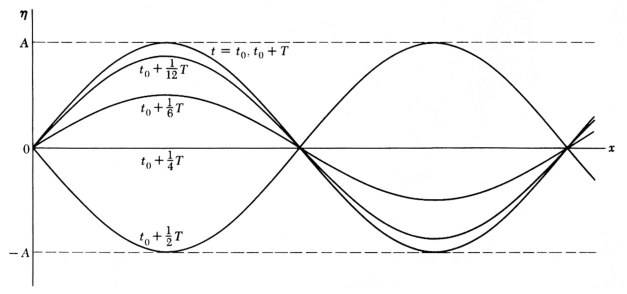
\includegraphics[height=2.5in]{../figs/L19/StandingWave}
  \caption{A standing wave shown at various times. (source:
    \textbf{EH} chap.~1)}
  \label{fig:standwave}
\end{figure}

The wave pattern represented by \autoref{eq:standwave} is called a
\textit{standing wave} because it does not advance along the string.
All the elements of the string oscillate in phase, and at any fixed
position, the string simply vibrates back and forth with the amplitude
$A\sin(\kappa x)$.  \autoref{eq:standwave} is plotted for various
times in \autoref{fig:standwave}.  The points with zero amplitude for
all $t$ are called \textit{nodes}.  If rigid boundaries are introduced
at any pair of nodes without changing the tension of the string, then
the standing-wave pattern is not altered.

What are all the possible standing-wave patterns that can exist on a
stretched string? (We covered this briefly in the last lecture of
Hilary term).  Suppose we fix the string with rigid boundaries at
$x=0$ and $x=l$.  For nodes to exist at these two points, it is
necessary that the wave number $\kappa$ have one of the following
values, indexed by the integer $n$
\begin{equation}
  \label{eq:2}
  \kappa_n = n\frac{\pi}{l},\;\;\;\text{with}\;\;\;n=1,2,3,...
\end{equation}
which makes $\sin(\kappa_n x)$ vanish at $x=l$.  The corresponding
resonant frequencies are
\begin{equation}
  \label{eq:4}
  \omega_n = c\kappa_n = n\frac{\pi c}{l} = n\omega_1,
\end{equation}
where $\omega_1 = \pi c/l$ is the \textit{fundamental} mode. The
frequencies of higher modes, also called \textit{overtones}, are
\textit{harmonics} (integer multiples) of the fundamental.  Because
the wave equation is linear, the entire family of permitted standing
waves can exist on the string simultaneously, each with arbitrary
(small) amplitude.  Each is independent of the others.


\subsection{The general motion of a finite string segment}

In this section we're again considering a segment of string that is
fixed at its ends, at $x=0,l$.  \EH{1.6} Last lecture we found that
each of the \textit{normal modes} of the segment is a standing wave
with nodes at the segment ends.  We can describe the entire family of
possible normal modes using a summation
\begin{equation}
  \label{eq:sumsoln}
  \eta(x,t) = \sum_{n=1}^\infty \sin(\kappa_nx)
  \left[a_n\cos(\omega_nt) + b_n\sin(\omega_nt)\right],
\end{equation}
where $a_n$ and $b_n$ are the amplitudes of the standing waves of
frequency $\omega_n$.  The frequencies and wavenumbers are related by
the equation $\omega_n = c\kappa_n$, with $\kappa_n$ determined by the
boundary conditions that give
\begin{displaymath}
  \kappa_n = n\pi/l,\;\;\;n=1,2,3,...
\end{displaymath}

Does \autoref{eq:sumsoln} look familiar?  It should!  It is a Fourier
series.  Recall that for diffusion, we wrote the initial condition as
a Fourier series summation, and then obtained its evolution with time
by multiplying each term by a decaying exponential with the
appropriate decay constant.  The diffusion equation is linear, and
hence each decaying mode was independent of the others.  The same is
true for the wave equation, which is also linear.  The initial
condition of the string can be decomposed into Fourier modes; each
Fourier mode evolves independently.  For the wave equation, however,
each Fourier mode \textit{oscillates} instead of decaying.  Let's see
how this works mathematically.

There are two ways to start the string vibrating: first, we could give
it an initial displacement, with no initial velocity (like plucking a
guitar string); second, we could give it an initial velocity, with no
initial displacement (like a piano hammer hitting a piano string).
We'll denote the initial displacement as $\eta_0(x)$ and the initial
velocity as $\dot{\eta}_0(x)$. Examining \autoref{eq:sumsoln} and
recalling the properties of sine and cosine functions, we can see that
in the case of zero initial displacement we have $a_n=0$, while for
zero initial velocity we have $b_n=0$.  In particular, we can write
the initial condition in terms of two Fourier series
\begin{align}
  \eta_0(x) &= \sum_{n=1}^\infty a_n\sin(\kappa_nx),\\
  \dot{\eta}_0(x) &= \sum_{n=1}^\infty b_n\omega_n\sin(\kappa_nx).
\end{align}
In the second equation, you will note the appearance of the
$\omega_n$. The dot in $\dot{\eta}_0$ indicates the time-derivative of
displacement; since \autoref{eq:sumsoln} represents the displacement,
we must take its time-derivative before setting $t=0$ and equating
with $\dot{\eta}_0(x)$.  In taking this derivative we obtain the
factor of $\omega_n$.

\paragraph{Example: plucked string}
As an example, let's consider a case with $\dot{\eta}_0(x)=0$.
Suppose a string is plucked to give the initial condition
\begin{equation}
  \label{eq:pluckedIC}
  \eta_0(x) =
  \begin{cases}
    \frac{2A}{l}x & \text{for $0\le x\le l/2$},\\
    \frac{2A}{l}(l-x) & \text{for $l/2 < x\le l$},
  \end{cases}
\end{equation}
as shown in the top panel of \autoref{fig:plucked}.

\begin{SCfigure}[1][ht]
  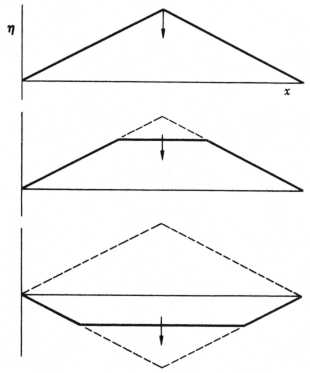
\includegraphics[height=3in]{../figs/L20/PluckedString}
  \caption{Initial condition and subsequent evolution of a plucked
    string.  (source: \textbf{EH} chap.~1)\vspace{1in}}
  \label{fig:plucked}
\end{SCfigure}

We have already established that all $b_n=0$ because the string has no
initial velocity.  To find $a_n$ we use the formula
\begin{align}
  a_n &= \frac{2}{2l}\int_0^{2l}\eta_0(x)\sin\frac{2\pi nx}{2l}\infd x,\nonumber\\
      &= \frac{2}{l}\int_0^{l}\eta_0(x)\sin\frac{\pi nx}{l}\infd x,
\end{align}
where we have taken the full period of oscillation as $2l$, and then
simplified the integral using symmetry properties of the initial
condition.  Substituting \autoref{eq:pluckedIC} gives the integral
\begin{displaymath}
  a_n = \frac{4A}{l}\left[\int_0^{l/2}\frac{x}{l}\sin\frac{\pi nx}{l}\infd x + 
    \int_{l/2}^l\left(1-\frac{x}{l}\right)\sin\frac{\pi nx}{l}\infd x\right].
\end{displaymath}
Using the tricks that you learned last term, this can be evaluated as
\begin{equation}
  \label{eq:4}
  a_n = \frac{8A}{\pi^2n^2}(-1)^{(n-1)/2},\;\;\;n=1,3,5,...
\end{equation}
Hence the initial shape of the string is given by the Fourier series
\begin{equation}
  \label{eq:5}
  \eta_0(x) = \frac{8A}{\pi^2}\left(\frac{1}{1^2}\sin\frac{\pi x}{l} - 
    \frac{1}{3^2}\sin\frac{3\pi x}{l} + ...\right).
\end{equation}
Referring back to the general solution \autoref{eq:sumsoln}, we can
write a formula for the displacement of the string at any later time
as
\begin{equation}
  \label{eq:6}
  \eta(x,t) = \frac{8A}{\pi^2}\left(\frac{1}{1^2}\sin\frac{\pi x}{l}\cos\omega_1t - 
    \frac{1}{3^2}\sin\frac{3\pi x}{l}\cos 3\omega_1t + ...\right),
\end{equation}
where $\omega_1 = c\kappa_1 = \pi c/l$ is the fundamental frequency
and $T_1 = 2\pi/\omega_1$ is the fundamental
period. \autoref{fig:plucked} shows the inital displacement of the
string, and subsequent displacements for $t>0$.

\subsection{Computing the evolution of an initial displacement with
  \Mlab}

As with diffusion, it is possible to use the discrete Fourier series
to compute the evolution of an initial displacement of the string.
This case is different, however, because we need to restrict our
series to only sine terms.  This is evident if you look back to
\autoref{eq:sumsoln} and set $t=0$.  It is also clear if you consider
that $\eta$ must always equal zero at its end-points, $x=0$ and $x=l$.

The following \Mlab function computes the sine series of an arbitrary
initial condition \texttt{eta0} (\textit{displacement only}!) and then
computes the displacement \texttt{eta} at times specified in the
vector \texttt{time}.  The first and last entries in \texttt{eta0}
must be zero, and there must be an even number of entries in vectors
\texttt{x} and \texttt{eta0}.

\verbatiminput{../figs/L20/dfs_stringwaves.m}

\begin{figure}[tb]
  \centering
  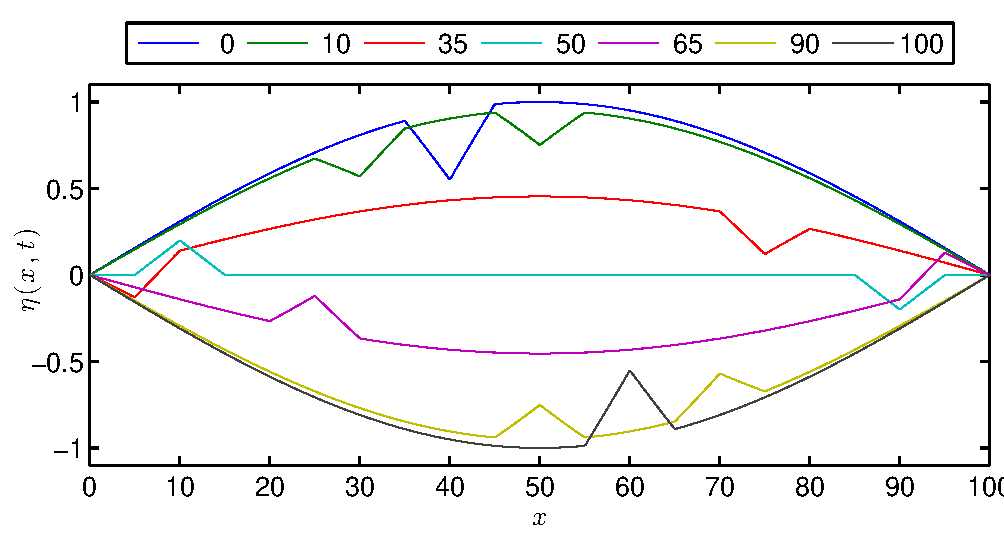
\includegraphics[height=2.5in]{../figs/L20/StringEvolution}
  \caption{Evolution of an initial displacement to a string, computed
    with \texttt{dfs\_stringwaves.m}.}
  \label{fig:stringevol}
\end{figure}

The evolution of a prescribed initial condition $\eta_0(x)$ (blue) is
shown in \autoref{fig:stringevol}.  Each line represents the solution
at a different time, up to $t=1$, which is one half of the fundamental
period.  This figure was generated with the following \Mlab commands:
\Minput{x = linspace(0,100,1000);} \Minput{eta0 = sin(pi*x/100) -
  interp1([0 35 40 45 100],[0 0 0.4 0 0],x);} \Minput{time = [0 10 35
  50 65 90 100];} \Minput{eta = dfs\_stringwaves(x,eta0,1,time);}
\Minput{p = plot(x,eta);} \Minput{legend(p,num2str(time'));}

\end{document}

%%% Local Variables:
%%% mode: latex
%%% TeX-master: t
%%% End:
